% =====================================================================
% CAPITOLO 5 — stesura della candidata, con le correzioni del 9 settembre.
%
% ATTENZIONE: e' ISS-110, questo NON e' `Cap5.tex` del repository.
% ATTENZIONE: il testo consegnato si interrompeva dentro il paragrafo
% sulla sospensione automatica, su «Al risveglio la registrazione
% riprendeva normalme». La coda e' stata RICOSTRUITA il 9 settembre:
% parole di chi ricostruisce, fatti presi da EXP-024 e da ISS-130/151.
% Il blocco in fondo dice esattamente che cosa e' stato scritto.
%
% ---------------------------------------------------------------------
% A. LA CORREZIONE PIU' GRANDE: `tab:costo` (§5.4.1)
%
% Il testo riportava 1,21 / 33,34 / 0,94 / 2,20 ms = 37,7 ms, 26,5 fps,
% 88,4% percezione e 5,8% classificatore. Sono i valori RITIRATI da
% ISS-137 il 6 settembre: erano trascritti da una sessione di terminale e
% nessun file li produceva.
%
% Il testo diceva anche: «al momento della stesura, la misura completa non
% e' stata ancora ripetuta durante una nuova prova prolungata sulla board».
% NON E' PIU' VERO: e' stata ripetuta il 6 settembre su 4,59 ore di
% esercizio continuo (EXP-024), e il registratore la scrive ora nel proprio
% riepilogo.
%
% Valori misurati: 0,25 / 116,38 / 0,50 / 19,51 = 136,65 ms, 7,3 fps,
% percezione 85,2%, classificatore 14,3%. Le quattro fasi sommano al totale
% con scarto 0,0000 ms: non c'e' overhead, come il relatore chiedeva di
% verificare al punto 8.
%
% Il relatore ha scritto: «Userei esclusivamente le nuove misure e
% toglierei dal testo principale i vecchi valori non riproducibili».
% Fatto: la tabella nuova e' quella principale, la vecchia resta come
% riquadro di confronto perche' la discordanza e' essa stessa un risultato.
%
% ---------------------------------------------------------------------
% B. `tab:latenza` (§5.6.2) — ISS-146
% L'addendo di calcolo valeva 0,038 s, cioe' i 37,7 ms ritirati. Alla
% cadenza vera vale 0,125 s: totale 3,865 s invece di 3,778, e il rapporto
% fra finestra e calcolo scende da «superiore a settanta» a VENTIDUE.
% Aggiunta `tab:latenza_sensibilita`, che isola i tre contributi.
%
% ---------------------------------------------------------------------
% C. IL FATTORE FINESTRE/EVENTI: 47,8 -> 44,8 (ISS-140)
% E il relatore ha segnalato l'apparente incoerenza fra il 44,8 aggregato e
% il 14,9 della figura. Non e' un errore: il rapporto NON e' costante,
% dipende da quanto sono lunghe le raffiche. Per sessione sta fra 12 e 15;
% il 44,8 e' un rapporto fra somme e lo dominano le sessioni con le raffiche
% piu' lunghe. Ora e' scritto, in didascalia e nel testo.
%
% ---------------------------------------------------------------------
% D. LA DURATA DI K (§5.7.3) — ISS-148
% Il testo diceva «a 9 fps, K=31 corrisponde a circa 3,4 s» e ne ricavava un
% campo di ricezione di 5,8 s. Ma K si applica in ESTRAZIONE, sullo stream
% pieno a 18 fps: sono 1,72 s, e il campo di ricezione 4,17 s. I 3,4 s
% sarebbero il valore se il dispositivo girasse a 9 fps; ne fa 7,26, e li'
% durano 4,27 s. E' il disallineamento fra addestramento ed esercizio, e va
% detto per quello che e'.
%
% ---------------------------------------------------------------------
% E. STRUTTURA: due coppie di sottosezioni erano titoli vuoti consecutivi
% (§5.4.1/5.4.2 e §5.5.1/5.5.2). Il testo che seguiva apparteneva alla
% prima; ora e' distribuito.
%
% F. Refusi: la frase d'apertura era senza principale; «riteri» ->
% «criteri»; il rimando ai 4,47 ms ora dichiara che sono del calcolatore.
% =====================================================================

\chapter{Implementazione su dispositivo edge e validazione in ambiente reale}
\label{cap:campo}
\label{cap:edge}

I capitoli precedenti hanno stabilito che cosa il sistema riconosce e con quale protocollo la misura sia difendibile. In questo capitolo vengono invece affrontati due aspetti complementari. Il primo riguarda l'implementazione della pipeline su un dispositivo edge, considerando compatibilità software, costo computazionale, frequenza di elaborazione e stabilità durante il funzionamento continuo. Il secondo riguarda la valutazione del sistema in ambiente domestico, dove cambiano la frequenza degli eventi, le attività osservate, il numero di persone presenti e le condizioni di ripresa.

\section{Piattaforma hardware e vincoli di porting}

L'hardware di riferimento è una \textbf{Radxa ROCK 4D}: SoC Rockchip RK3576, 6~GB di memoria, e un acceleratore neurale integrato da 6~TOPS. Il costo è dell'ordine del centinaio di euro, telecamera USB compresa.

\begin{table}[ht]
\centering
\caption{Le due architetture possibili per un sistema domestico. La riga che
decide non è il costo ma l'ultima: quali dati lasciano l'abitazione.}
\label{tab:edge_vs_server}
\begin{tabular}{lll}
\toprule
 & Nodo \emph{edge} & Server con GPU \\
\midrule
Calcolo & SoC ARM + NPU 6 TOPS & CPU x86 + GPU dedicata \\
Costo per stanza & $\sim$100 € & migliaia di € (condiviso) \\
Rete richiesta & nessuna & flusso video continuo \\
Dati in uscita & solo allarmi & fotogrammi \\
\bottomrule
\end{tabular}
\end{table}

La differenza che conta non è il prezzo assoluto ma il \textbf{costo per stanza}. Un server si ammortizza su molte telecamere, ma richiede che ogni telecamera gli mandi il proprio flusso: la scala abbatte il costo di calcolo e moltiplica quello di rete, e soprattutto sposta fuori dall'abitazione dati che il Capitolo~\ref{cap:contesto} ha argomentato debbano restarci. Un nodo autonomo per stanza non ha economia di scala, ma il suo costo marginale è noto e la sua superficie di esposizione è nulla.

\medskip

Il porting ha incontrato tre difficoltà, riportate perché un lavoro puramente simulativo non le incontra e documentarle è parte del contributo di un capitolo sul \emph{deployment}. Hanno una proprietà in comune: nessuna delle tre produce un messaggio d'errore che indichi la causa.

\begin{itemize}

\item \textbf{L'architettura del processore.} Il RK3576 implementa ARMv8.0. I pacchetti MediaPipe recenti sono compilati per ARMv8.1 e usano le istruzioni atomiche LSE, assenti nel set precedente: l'esecuzione termina con \texttt{illegal instruction}, senza alcun messaggio che indichi la causa reale. L'unica versione funzionante è la 0.10.9.

\item \textbf{La rimozione di un'API.} MediaPipe 1.0 ha eliminato \texttt{mp.solutions}, l'interfaccia impiegata dal codice di estrazione. Aggiornare avrebbe comportato riscrivere l'intera catena di feature e, con essa, invalidare il confronto con tutte le misure precedenti. La versione è stata quindi congelata, ed è una decisione da dichiarare: il sistema è vincolato a una libreria che gli autori considerano superata.

\item \textbf{La forma statica del modello accelerato.} Il modello convertito per l'NPU accetta un tensore di forma fissa a quattro dimensioni. Fornendone uno a tre dimensioni non si ottiene alcun errore: l'inferenza semplicemente non viene eseguita, e la funzione restituisce in tempi bassissimi. È l'origine di uno degli episodi discussi nella sezione seguente.

\end{itemize}

\section{Verifica di equivalenza fra calcolatore e dispositivo}
\label{sec:parita}

Prima di misurare le prestazioni computazionali della pipeline sul dispositivo è necessario verificare che il modello produca gli stessi risultati ottenuti sul calcolatore utilizzato per lo sviluppo. Una differenza nelle versioni delle librerie, nell'ordine delle feature o nella normalizzazione potrebbe infatti produrre un sistema formalmente funzionante ma non equivalente a quello valutato nel Capitolo~\ref{cap:risultati}.

La prima verifica viene effettuata su 200 finestre temporali precalcolate. Queste attraversano la stessa normalizzazione e lo stesso classificatore utilizzati durante l'inferenza, e le probabilità prodotte sul calcolatore vengono confrontate con quelle ottenute sulla board.

\begin{table}[ht]
\centering
\caption{Verifica di equivalenza del classificatore su 200 finestre
precalcolate.}
\label{tab:parita}
\begin{tabular}{lr}
\toprule
Scarto massimo sulle predizioni & $2{,}2\times10^{-16}$ \\
Campioni divergenti & 0 \\
\bottomrule
\end{tabular}
\end{table}

È la precisione della rappresentazione in virgola mobile: i due sistemi sono numericamente identici. La stessa verifica, ripetuta sul pacchetto multi-persona, ha dato scarto massimo esattamente nullo.

Va però dichiarato che cosa questa verifica \emph{non} copre. Le duecento finestre sono precalcolate: il confronto parte dalle grandezze geometriche e non dall'immagine, e quindi \textbf{non attraversa lo stimatore di posa}. Poiché MediaPipe Pose è un tracciatore e mantiene stato fra fotogrammi, il suo comportamento può divergere fra architetture diverse anche a parità di versione. La verifica di equivalenza qui riportata è quindi una verifica del \emph{classificatore}, non dell'intera catena percettiva; una verifica che parta dai fotogrammi richiede di conservare le immagini, ed è discussa fra i limiti alla fine del capitolo.

\paragraph{Perché la verifica viene prima, e non dopo.}

Questo controllo può sembrare una formalità. Non lo è, e la ragione è che nel corso del lavoro \textbf{tre misure distinte hanno riportato come successo il proprio fallimento}, in forme diverse e tutte plausibili a prima vista.

\begin{enumerate}

\item \textbf{Latenze identiche fra configurazioni diverse.} Quattro modelli di dimensione molto diversa producevano tempi indistinguibili. Il motivo era che nessuna persona veniva rilevata nei fotogrammi di prova: si stava cronometrando il ramo vuoto, quello che si percorre quando non c'è nulla da elaborare.

\item \textbf{1315 fotogrammi al secondo dichiarati.} Un valore fuori scala di due ordini di grandezza rispetto a qualunque aspettativa. L'input aveva tre dimensioni invece di quattro e l'inferenza non partiva affatto: il cronometro misurava il tempo di una funzione che ritornava senza fare nulla.

\item \textbf{«Nove keypoint su nove trovati»}, con le ginocchia disegnate sul torace. Il criterio di validità era $x > 0$ e $y > 0$, senza alcun controllo sulla confidenza: qualunque coordinata numericamente lecita veniva contata come rilevamento riuscito.

\end{enumerate}

Tutti e tre gli episodi condividono una struttura: \emph{il sistema non ha svolto il lavoro, e la misura ha riportato un risultato eccellente.} Un cronometro non distingue fra un'operazione veloce e un'operazione non eseguita, e un contatore non distingue fra un rilevamento corretto e un valore che sta nell'intervallo giusto per caso.

\begin{quote}
Un banco di prova che non verifica di aver svolto il lavoro misura il proprio fallimento e lo riporta come successo.
\end{quote}

Ne segue una regola operativa che questo lavoro ha adottato dopo il secondo episodio e mantenuto fino alla fine: \textbf{la verifica di equivalenza precede sempre la verifica di velocità}, e nessuna misura di prestazione viene accettata prima che sia stato dimostrato che il calcolo è avvenuto.

\section{Confronto fra stimatori di posa e configurazione operativa}
\label{sec:npu}

Con lo stimatore di partenza eseguito sulla CPU il dispositivo non regge il carico. Questa sezione descrive la strada percorsa per farlo reggere --- portare la percezione sull'acceleratore neurale, il che comporta cambiare stimatore --- e si chiude con la decisione di non percorrerla.

Occupa lo spazio che occupa perché il lavoro speso per ottenere quel risultato negativo è stato consistente, e perché una scelta verificata e smentita è un risultato, mentre una scelta assunta e mai messa alla prova non lo è.

\subsection{Valutazione dello stimatore accelerato}

L'arco di questa sottosezione va da una constatazione a una misura di ritenzione delle pose, e cambia segno a metà: l'acceleratore fa guadagnare il tempo che serve, e lo stimatore che permette di usarlo non trova le persone distese --- che sono l'unica cosa che questo sistema deve vedere.

\paragraph{Il punto di partenza non è utilizzabile.}

MediaPipe eseguito sulla CPU del dispositivo impiega \textbf{92,6~ms per fotogramma} a livello di sistema, cioè \textbf{10,8~fps}. Il Capitolo~\ref{cap:risultati} ha misurato che a 9~fps le cadute non rilevate raddoppiano rispetto ai 18~fps del dataset: la configurazione di partenza è quindi già sotto la soglia, e non è una base su cui costruire.

\paragraph{Il guadagno dell'acceleratore, e dove finisce.}

Sostituendo lo stimatore con YOLOv8-pose~\cite{yolopose} quantizzato ed eseguito sull'NPU, la \emph{sola inferenza} risulta \textbf{5,16 volte} più veloce. Ma la misura a livello di sistema dà \textbf{1,71}, non 5,16.

La differenza sta nella post-elaborazione: la decodifica dell'uscita e la soppressione dei rilevamenti ridondanti, scritte in Python con cicli espliciti, costavano \textbf{12,14~ms} --- più di un terzo del tempo totale. Riscritte in forma vettoriale scendono a \textbf{0,94~ms}, cioè \textbf{12,9 volte}, e il guadagno di sistema sale a 2,17.

È un esempio istruttivo di \textbf{collo di bottiglia che si sposta}: accelerando la componente più costosa se ne rende dominante una che prima era invisibile. Il primo numero, 5,16, non era sbagliato --- misurava esattamente ciò che dichiarava di misurare --- ma rispondeva a una domanda diversa da quella che interessava.

\paragraph{YOLOv8 non localizza una persona distesa.} È la parte che ribalta la conclusione della sezione, ed è interessante proprio perché il risultato è negativo. Ritenzione delle pose per tipo di attività, su 29.681 fotogrammi:

\begin{table}[ht]
\centering
\caption{Quota di \emph{landmark} ritenuti dai due stimatori, per attività. Il
divario si apre solo sulle posture prossime al suolo, che sono quelle che
contano. Impianto a cinque soggetti.}
\label{tab:ritenzione}
\begin{tabular}{lrr}
\toprule
Attività & YOLOv8 INT8 & MediaPipe \\
\midrule
In piedi, sedersi, raccogliere, saltare & 100\% & 100\% \\
Caduta in avanti sulle mani & 79,2\% & 99,5\% \\
\textbf{Stare sdraiati} & \textbf{43,6\%} & \textbf{79,1\%} \\
\bottomrule
\end{tabular}
\end{table}

Su tutto ciò che accade in piedi i due stimatori sono indistinguibili. Il divario si apre \textbf{solo sui corpi orizzontali} --- cioè esattamente sulla fase post-caduta, che è la più lunga e la più informativa.

\paragraph{Non è una questione di soglia.} L'obiezione naturale è che basti abbassare la confidenza minima. È stata verificata: scendendo a $0{,}05$, la ritenzione su «stare sdraiati» arriva al 58,9\%, ancora venti punti sotto MediaPipe. Il rilevatore non è prudente, semplicemente non trova la persona.

\paragraph{E dove la trova, la misura male.} La lunghezza del torso proiettata passa da 83,5 a 56,5 pixel fra la postura eretta e quella a terra, cioè $-32\%$; con MediaPipe va da 83,8 a 100,7. Su una telecamera laterale un torso che si distende \emph{non deve accorciarsi}: l'avvicinamento alla telecamera semmai lo allunga.

Il punto è che \texttt{torso\_len} è il \textbf{denominatore dell'intera normalizzazione body-centric}. Un suo errore non resta locale: si propaga a ogni feature del vettore, ed è sistematico e correlato con la classe --- cioè la forma di errore peggiore possibile, perché imita il segnale che si vuole misurare.

\paragraph{Il confronto a parità di protocollo.} Le due catene sono state infine confrontate variando soltanto lo stimatore di posa: stessa validazione, stesso insieme di grandezze, stesso modello, stessa soglia. È l'unico confronto della sezione in cui il divario supera nettamente la dispersione, e per questo è quello su cui la decisione si regge.

\emph{Provenienza dei valori di $F_2$.} I confronti di prestazione riportati in questa sezione provengono dall'impianto a \textbf{cinque} soggetti e non sono stati ripetuti dopo l'estensione a dieci. Le misure di \emph{tempo} --- millisecondi per fotogramma, ripartizione del costo, frequenza raggiunta --- non ne dipendono, perché sono state prese sul dispositivo e non su un insieme di verifica: quelle restano valide come sono. I valori di $F_2$ vanno invece letti come indicativi.

\begin{table}[ht]
\centering
\caption{Prestazione a parità di protocollo con i due stimatori di posa.
Impianto a cinque soggetti; le dispersioni sono deviazioni standard fra i fold.}
\label{tab:stimatori_f2}
\begin{tabular}{lrrr}
\toprule
Stimatore & $F_2$ & Falsi positivi & Falsi negativi \\
\midrule
MediaPipe & \textbf{0,909 $\pm$ 0,095} & \textbf{17} & \textbf{23} \\
YOLOv8 INT8 & 0,682 $\pm$ 0,044 & 225 & 59 \\
\bottomrule
\end{tabular}
\end{table}

Il divario è di \textbf{0,227}, molto fuori dalle deviazioni: è una delle poche differenze misurate in questo lavoro che \emph{non} cada dentro il rumore.

\subsection{Scelta della configurazione operativa}
\label{sec:decisione}

Questa parte del capitolo non si conclude dichiarando che il sistema gira sull'acceleratore a 26,5~fps. Si conclude con una scelta motivata dai numeri, e la scelta è \textbf{contraria alla direzione seguita per ottenerli}.

Il confronto onesto non è a parità di dati ma a \textbf{parità di condizioni operative}: ciascuna catena valutata al frame rate che raggiunge davvero sul dispositivo.

\begin{table}[ht]
\centering
\caption{Le tre catene candidate: quella accurata non gira, quella veloce
perde troppo. La riga in grassetto è quella installata. Impianto a cinque
soggetti.}
\label{tab:catene}
\begin{tabular}{llrrr}
\toprule
Catena & Sul dispositivo & $F_2$ & FP & FN \\
\midrule
MediaPipe @ 18 fps & non raggiungibile & 0,898 & 23 & 24 \\
\textbf{MediaPipe @ 9 fps} & \textbf{10,8 fps} & \textbf{0,857} & \textbf{57} & \textbf{49} \\
YOLOv8 @ 18 fps & 26,5 fps & 0,682 & 225 & 59 \\
\bottomrule
\end{tabular}
\end{table}

\textbf{MediaPipe sottocampionato batte YOLOv8 a piena velocità di 0,175}, e lo batte su ogni voce: recall $0{,}866$ contro $0{,}775$, falsi negativi 49 contro 59, falsi allarmi 57 contro 225.

I due costi, messi accanto:

\begin{table}[ht]
\centering
\caption{Il costo delle due rinunce possibili, misurato. Cambiare stimatore
costa cinque volte più che dimezzare la frequenza dei fotogrammi, ed è la
ragione per cui l'acceleratore neurale non viene usato.}
\label{tab:scomposizione}
\begin{tabular}{lr}
\toprule
Sottocampionare MediaPipe da 18 a 9 fps & $-0{,}041$ \\
Cambiare stimatore di posa & $-0{,}216$ \\
\midrule
Rapporto & $5{,}3\times$ \\
\bottomrule
\end{tabular}
\end{table}

\textbf{Rinunciare a metà del frame rate costa cinque volte meno che rinunciare allo stimatore.} Il sistema va quindi costruito su MediaPipe, con il modello addestrato alla frequenza che il dispositivo regge davvero, così che addestramento ed esercizio coincidano.

Il costo va dichiarato e non attenuato: le cadute non rilevate passano dal 9,6\% al 13,4\% in questo impianto a cinque soggetti. La misura corrispondente sui dieci soggetti, riportata nel Capitolo~\ref{cap:risultati}, dà 6,8\% e 12,4\%; le due non sono confrontabili cifra per cifra perché provengono da impianti sperimentali diversi, ma indicano lo stesso ordine di peggioramento.

\paragraph{Che cosa resta del lavoro sull'acceleratore.}

La velocità dell'NPU è reale e misurata: $12{,}9\times$ sulla post-elaborazione, 26,5~fps a sistema. Non è quel lavoro a essere in discussione, ma il rapporto fra ciò che fa guadagnare e ciò che fa perdere \emph{su questo compito}.

Resta la strada più promettente se il divario dello stimatore si chiude, e le tre vie sono note:

\begin{itemize}
\item un modello di dimensione superiore al più piccolo della famiglia;
\item un confronto in virgola mobile contro la versione quantizzata a 8 bit, per \textbf{isolare la quantizzazione} --- che oggi non è isolata, ed è un limite da dichiarare: non si sa quanta parte dei 0,227 sia dovuta alla rete e quanta alla quantizzazione;
\item il rilevamento del contesto --- dove sono i mobili --- che su un rilevatore di oggetti sarebbe quasi gratuito, perché il secondo modello serve comunque.
\end{itemize}

\section{Prestazioni computazionali e affidabilità del dispositivo}

\subsection{Costo computazionale e frequenza di elaborazione}
\label{sec:costo}

Il confronto precedente mostra che la stima della posa costituisce il vincolo principale per la scelta della configurazione operativa. Per quantificare il peso delle diverse fasi la pipeline è stata strumentata, separando pre-elaborazione, percezione, post-elaborazione e classificazione.

\paragraph{Come è stata effettuata la misura.} I tempi sono rilevati con quattro letture di orologio monotono attorno alle quattro fasi, \emph{all'interno dell'esecuzione reale} e non in un banco separato: sono quindi i tempi della stessa esecuzione che ha prodotto gli allarmi della sessione. La misura copre \textbf{4,59 ore di esercizio continuo}, \textbf{119.928 fotogrammi} e una telecamera USB collegata, con persone che entrano ed escono dalla scena. Il tempo di acquisizione del fotogramma dalla telecamera è incluso nella pre-elaborazione; l'avvio della sessione, comprendente il caricamento del modello e le verifiche di equivalenza, è escluso. La strumentazione stessa costa quattro letture di orologio per fotogramma.

\begin{table}[ht]
\centering
\caption{Ripartizione del costo per fotogramma, misurata sul dispositivo
durante 4,59 ore di esercizio continuo. Le quattro fasi sommano al totale
senza residuo: non è presente overhead non attribuito.}
\label{tab:costo}
\begin{tabular}{lrr}
\toprule
\textbf{Fase} & \textbf{Tempo} & \textbf{Quota} \\
\midrule
Pre-elaborazione & 0,25 ms & 0,2\% \\
\textbf{Percezione} & \textbf{116,38 ms} & \textbf{85,2\%} \\
Post-elaborazione & 0,50 ms & 0,4\% \\
Classificatore, costo ammortizzato & 19,51 ms & 14,3\% \\
\midrule
\textbf{Totale} & \textbf{136,65 ms} & \textbf{7,3 fps} \\
\bottomrule
\end{tabular}
\end{table}

Il dato più importante riguarda la distribuzione del costo: \textbf{la percezione occupa l'85,2\% del tempo totale, mentre il classificatore rappresenta il 14,3\%}. Il classificatore --- l'oggetto su cui si concentra la letteratura, e su cui si è concentrato il Capitolo~\ref{cap:risultati} --- è quindi circa un settimo del problema.

\paragraph{Una misura precedente, ritirata.} Fino al 5 settembre 2026 questo capitolo riportava una ripartizione differente: 1,21 / 33,34 / 0,94 / 2,20~ms, per un totale di 37,7~ms e 26,5~fps, con la percezione all'88,4\% e il classificatore al 5,8\%. Quei valori erano stati ottenuti durante un banco dedicato e \emph{trascritti da una sessione di terminale}: nessun file li produceva, e non erano quindi riproducibili. La misura riportata nella Tabella~\ref{tab:costo} li sostituisce.

La discordanza è di un fattore \textbf{3,6} sui valori assoluti, e va riportata per intero. \emph{Reggono le proporzioni}: la percezione resta la voce dominante e il classificatore la voce marginale, quindi l'affermazione portante del capitolo non cambia, e non cambia la conseguenza --- la scelta del classificatore non determina la frequenza di esercizio. \emph{Non reggono i valori assoluti}, e un indizio era già presente nel progetto: il file di configurazione dichiara da sempre che il dispositivo regge circa nove fotogrammi al secondo, ed è su quel presupposto che il dataset viene sottocampionato in addestramento. I 7,3~fps misurati sono coerenti con quel presupposto; i 26,5 dichiarati non lo erano mai stati, e i due numeri non erano mai stati confrontati fra loro.

L'obiezione immediata era che la misura fosse stata presa a stanza vuota, dove lo stimatore lavora in modo diverso. È stata verificata, ed era sbagliata: ripetuta con un soggetto in scena il costo \emph{sale} da 126,0 a 144,1~ms su una prova di un minuto, perché al rilevatore di persone si aggiunge il modello dei landmark. Il divario si allarga invece di chiudersi.

\paragraph{Una nota sulle unità.} Il costo del classificatore compare nell'elaborato con due unità diverse, e la differenza va spiegata perché altrimenti sembra una discordanza. Le finestre avanzano con passo pari a due, quindi il classificatore viene eseguito una volta ogni due fotogrammi: il costo per \emph{finestra} è circa il doppio di quello per \emph{fotogramma}. Sulla misura del 6 settembre i due valori sono 39,04~ms per finestra e 19,51~ms per fotogramma.

Il Capitolo~\ref{cap:risultati} riporta inoltre un costo di 4,47~ms per finestra. \textbf{Quella è una misura effettuata sul calcolatore di sviluppo, non sul dispositivo}, ed è coerente con il controllo indipendente che sullo stesso calcolatore dà 4,85~ms mediani per la Random Forest. Sul dispositivo lo stesso classificatore costa circa otto volte tanto. I due valori non vanno quindi messi sulla stessa scala.

La Random Forest non è dunque il classificatore più veloce fra quelli considerati: la sua scelta è legata soprattutto alla semplicità di deployment, al tempo di addestramento ridotto e all'assenza della dipendenza da TensorFlow sul dispositivo. La caratterizzazione temporale mostra comunque che, anche sostituendo il classificatore con un modello sensibilmente più veloce, il guadagno sulla pipeline completa sarebbe limitato: il principale margine di ottimizzazione rimane nella fase di percezione.

\subsection{Stabilità termica e continuità operativa}
\label{sec:termico}

La stabilità del dispositivo è stata verificata sotto carico continuo. In una prova di dieci minuti, comprendente 18.291 inferenze, la variazione della latenza fra l'inizio e la fine è stata pari a circa il 3,9\%. La frequenza dell'acceleratore è rimasta a 950~MHz e la temperatura si è stabilizzata fra 60 e 63~$^\circ$C, senza evidenza di riduzioni improvvise della frequenza di elaborazione.

Una verifica più lunga è stata ottenuta durante una sessione domestica. Nel corso di circa cinque ore la temperatura massima registrata è stata pari a 79,5~$^\circ$C e l'andamento ha raggiunto un regime dopo circa quaranta minuti. Non sono stati osservati cali improvvisi del frame rate riconducibili a \emph{thermal throttling}. L'assenza di gradini è il criterio adottato: un dispositivo che si rallenta da solo mostra cali bruschi, non una deriva lenta.

Queste misure indicano che la temperatura non costituisce, nelle prove effettuate, il principale limite al funzionamento continuo. Come verrà mostrato nelle sezioni successive, i problemi emersi durante le sessioni prolungate riguardano invece soprattutto la gestione del flusso video, la sospensione del sistema e le condizioni reali della scena.

\bigskip

Le verifiche precedenti riguardano il funzionamento della pipeline sul dispositivo e il costo necessario per elaborare il flusso video. Rimane però da verificare un aspetto differente: come si comporta lo stesso sistema quando viene lasciato in funzione per diverse ore in un ambiente domestico, durante attività che non sono state costruite appositamente per il dataset.

\section{Validazione in ambiente domestico}

\subsection{Motivazione della valutazione in campo}
\label{sec:perche-non-basta}

Le metriche ottenute su un dataset descrivono il comportamento del sistema all'interno della distribuzione rappresentata dal dataset stesso. In una possibile applicazione domestica cambia però soprattutto la frequenza degli eventi: per quasi tutto il tempo non si verifica alcuna caduta e il sistema deve distinguere l'evento di interesse da un numero molto elevato di normali attività quotidiane.

Questo aspetto rende particolarmente importante il tasso di falsi positivi. Nella configurazione utilizzata prima delle sessioni domestiche il classificatore produceva circa 46 falsi positivi su 4767 finestre negative, corrispondenti a circa lo \textbf{0,96\%} delle decisioni. Su un dataset questo valore può essere compatibile con una buona precision, perché la quota di esempi positivi è artificialmente molto maggiore di quella osservabile durante un funzionamento reale.

Se lo stesso tasso viene proiettato su un giorno di funzionamento continuo, il numero di decisioni diventa molto elevato.

\begin{table}[ht]
\centering
\caption{Stima del numero di falsi positivi ottenibile durante un giorno di
funzionamento continuo mantenendo invariato il tasso per finestra osservato in
laboratorio.}
\label{tab:finestratura}
\begin{tabular}{lrr}
\toprule
\textbf{Finestratura} & \textbf{Finestre/giorno} &
\textbf{Falsi positivi/giorno} \\
\midrule
Non sovrapposta & $\sim34\,560$ & $\sim332$ \\
Con finestre sovrapposte & $\sim311\,000$ & $\sim2990$ \\
\bottomrule
\end{tabular}
\end{table}

La stima corrisponde a un intervallo compreso indicativamente fra \textbf{14 e 125 segnalazioni all'ora}. Il calcolo non rappresenta una previsione precisa del comportamento domestico, ma mostra che un tasso per finestra apparentemente ridotto può diventare problematico quando il sistema produce decisioni in modo continuo. Questa previsione è stata formulata \emph{prima} della prima sessione, ed è importante che venga letta in quest'ordine: una previsione registrata dopo i fatti non è una previsione.

\subsection{Protocollo delle sessioni domestiche}
\label{sec:protocollo-campo}

Per verificare direttamente questo comportamento sono stati registrati dodici blocchi distribuiti su quattro giornate e due abitazioni, per una durata complessiva pari a circa 9,6 ore. Le registrazioni comprendono periodi di vita quotidiana, prove di caduta simulate e attività scelte appositamente per verificare i casi più ambigui, come sedersi rapidamente, chinarsi, sdraiarsi volontariamente o avere più persone contemporaneamente nell'inquadratura. I partecipanti sono familiari dello studente, informati e consenzienti.

La telecamera viene posizionata lateralmente rispetto alla zona principale di movimento, seguendo il risultato ottenuto nella Sezione~\ref{sec:viewpoint}. L'asse ottico viene mantenuto approssimativamente orizzontale e la telecamera viene collocata a circa 1,2--1,5~m da terra. La distanza viene scelta in modo da mantenere all'interno dell'inquadratura sia la postura eretta sia la persona distesa sul pavimento o su una superficie rialzata.

\begin{figure}[htbp]
\centering
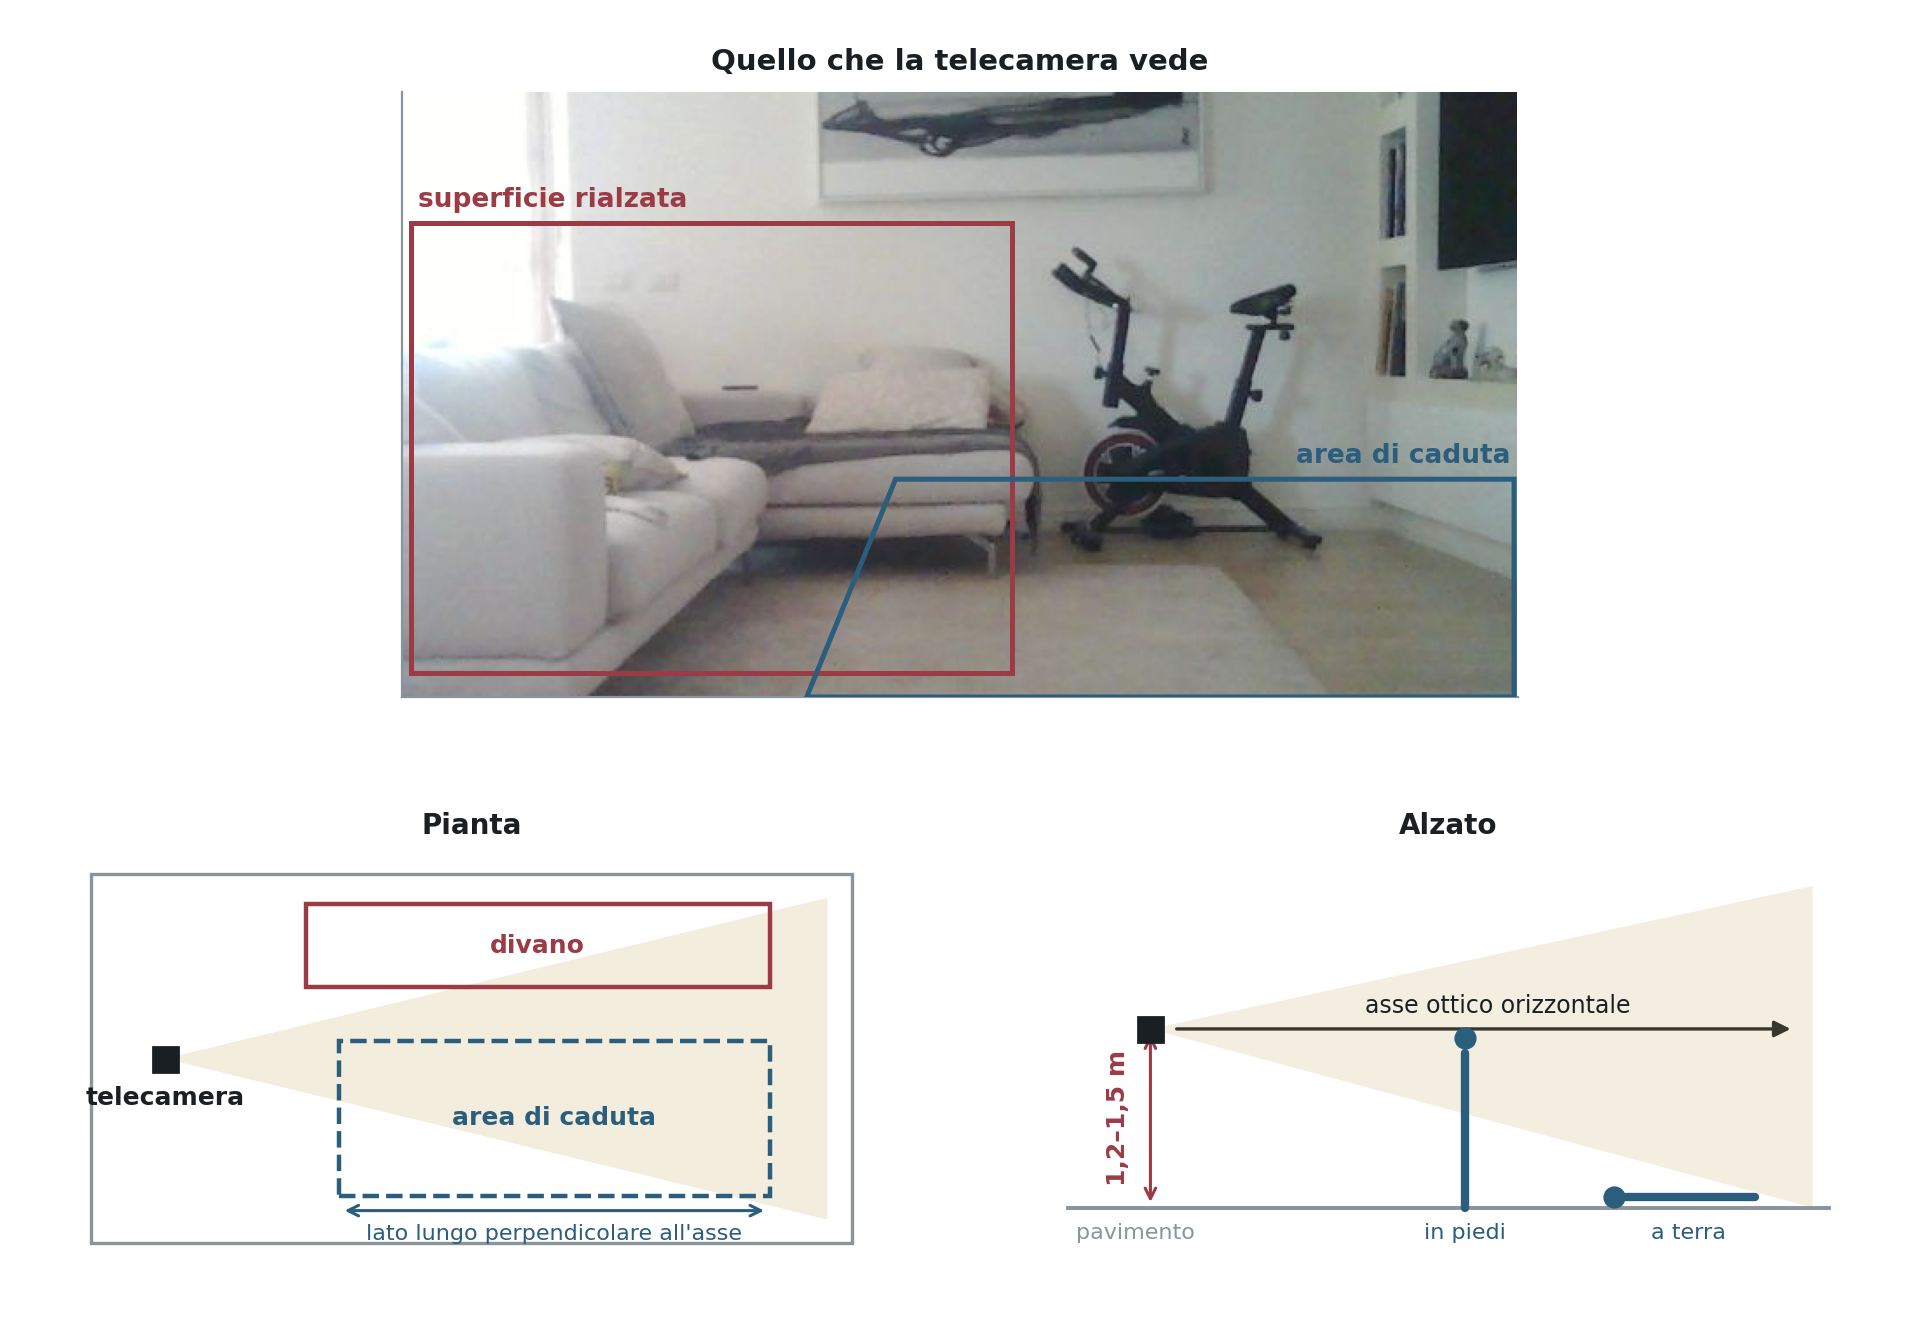
\includegraphics[width=.96\textwidth]{figure/fig_stanza.png}
\caption{Schema del posizionamento utilizzato per le acquisizioni domestiche.
L'inquadratura deve comprendere sia l'area in cui può avvenire la caduta sia
le superfici sulle quali una persona può trovarsi distesa durante le normali
attività. Si tratta di uno schema del protocollo di ripresa e non di dati
misurati.}
\label{fig:stanza}
\end{figure}

Il registratore salva in modo continuo soltanto i dati necessari all'elaborazione, come posa, feature e punteggi del classificatore. Le immagini RGB vengono mantenute sul dispositivo soltanto in prossimità delle segnalazioni, per permettere l'analisi degli errori. Il flusso video completo non viene quindi trasmesso né conservato in modo continuo. È il \emph{privacy-by-design} argomentato nel Capitolo~\ref{cap:contesto} dimostrato in pratica invece che dichiarato, e ha richiesto di rimuovere dal prototipo una registrazione video continua aggiunta per comodità di sviluppo, che contraddiceva l'argomento stesso della tesi.

Le cadute simulate vengono eseguite soltanto dai partecipanti per i quali la prova non presenta un rischio particolare. I partecipanti anziani non vengono invitati a eseguire cadute; nelle loro registrazioni sono presenti esclusivamente attività quotidiane. Di conseguenza, le cadute utilizzate per la misura del richiamo non appartengono alla popolazione anziana alla quale il sistema sarebbe principalmente destinato. Questo costituisce un limite della validazione.

Un secondo controllo riguarda la qualità della posa ottenuta nelle singole sessioni.

\begin{table}[ht]
\centering
\caption{Quota di fotogrammi con posa valida nelle giornate di acquisizione.}
\label{tab:qualita_sessioni}
\begin{tabular}{lll}
\toprule
\textbf{Giornata} & \textbf{Luogo} & \textbf{Pose valide} \\
\midrule
10 agosto & prima abitazione & 0,6--39,8\% \\
11 agosto & prima abitazione & 83,0\% \\
12 agosto & seconda abitazione & 86,8--99,3\% \\
13 agosto & seconda abitazione & 25,9--97,6\% \\
\bottomrule
\end{tabular}
\end{table}

Le sei registrazioni del 10 agosto presentano una quota di pose valide troppo bassa per poter misurare il classificatore. La telecamera era troppo vicina e una parte del corpo usciva frequentemente dall'inquadratura. Queste sessioni non vengono quindi utilizzate per calcolare i risultati quantitativi successivi, ma sono state utili per definire il protocollo di posizionamento della telecamera.

Anche una registrazione non utilizzabile dal punto di vista della classificazione fornisce quindi un'informazione importante: prima di valutare il modello è necessario verificare che la persona sia effettivamente osservabile durante entrambe le condizioni, in piedi e a terra. Va segnalato che \textbf{la sessione da cui provengono tutte e cinque le cadute annotate ha il 25,9\% di pose valide}, una quota inferiore a quella di sessioni che sono state scartate: il richiamo di campo riportato più avanti va letto tenendo conto di questo.

\section{Metriche di evento e prestazioni di sistema}
\label{sec:falsi-allarmi}
\label{sec:finestre-eventi}

Il classificatore produce una probabilità per ciascuna finestra temporale, ma un sistema installato non dovrebbe generare un nuovo allarme per ogni finestra consecutiva che supera la soglia. Una singola caduta o una singola attività ambigua può infatti mantenere il punteggio elevato per più finestre sovrapposte.

Contare ciascuna di queste finestre come un evento porterebbe quindi a sovrastimare fortemente il numero di segnalazioni percepite dall'utente. Sull'insieme delle registrazioni effettuate, il rapporto fra il numero complessivo di finestre sopra soglia e il numero complessivo di eventi di allarme vale \textbf{44,8}.

Per trasformare le decisioni sulle finestre in eventi viene utilizzata una regola di persistenza. Un allarme viene generato quando almeno cinque finestre consecutive superano la soglia decisionale. Dopo l'emissione viene applicato un intervallo di sospensione di 30~s, durante il quale eventuali ulteriori finestre positive vengono considerate parte dello stesso episodio.

La Figura~\ref{fig:sessione} mostra un esempio di questa differenza su una sessione prolungata.

\begin{figure}[htbp]
\centering
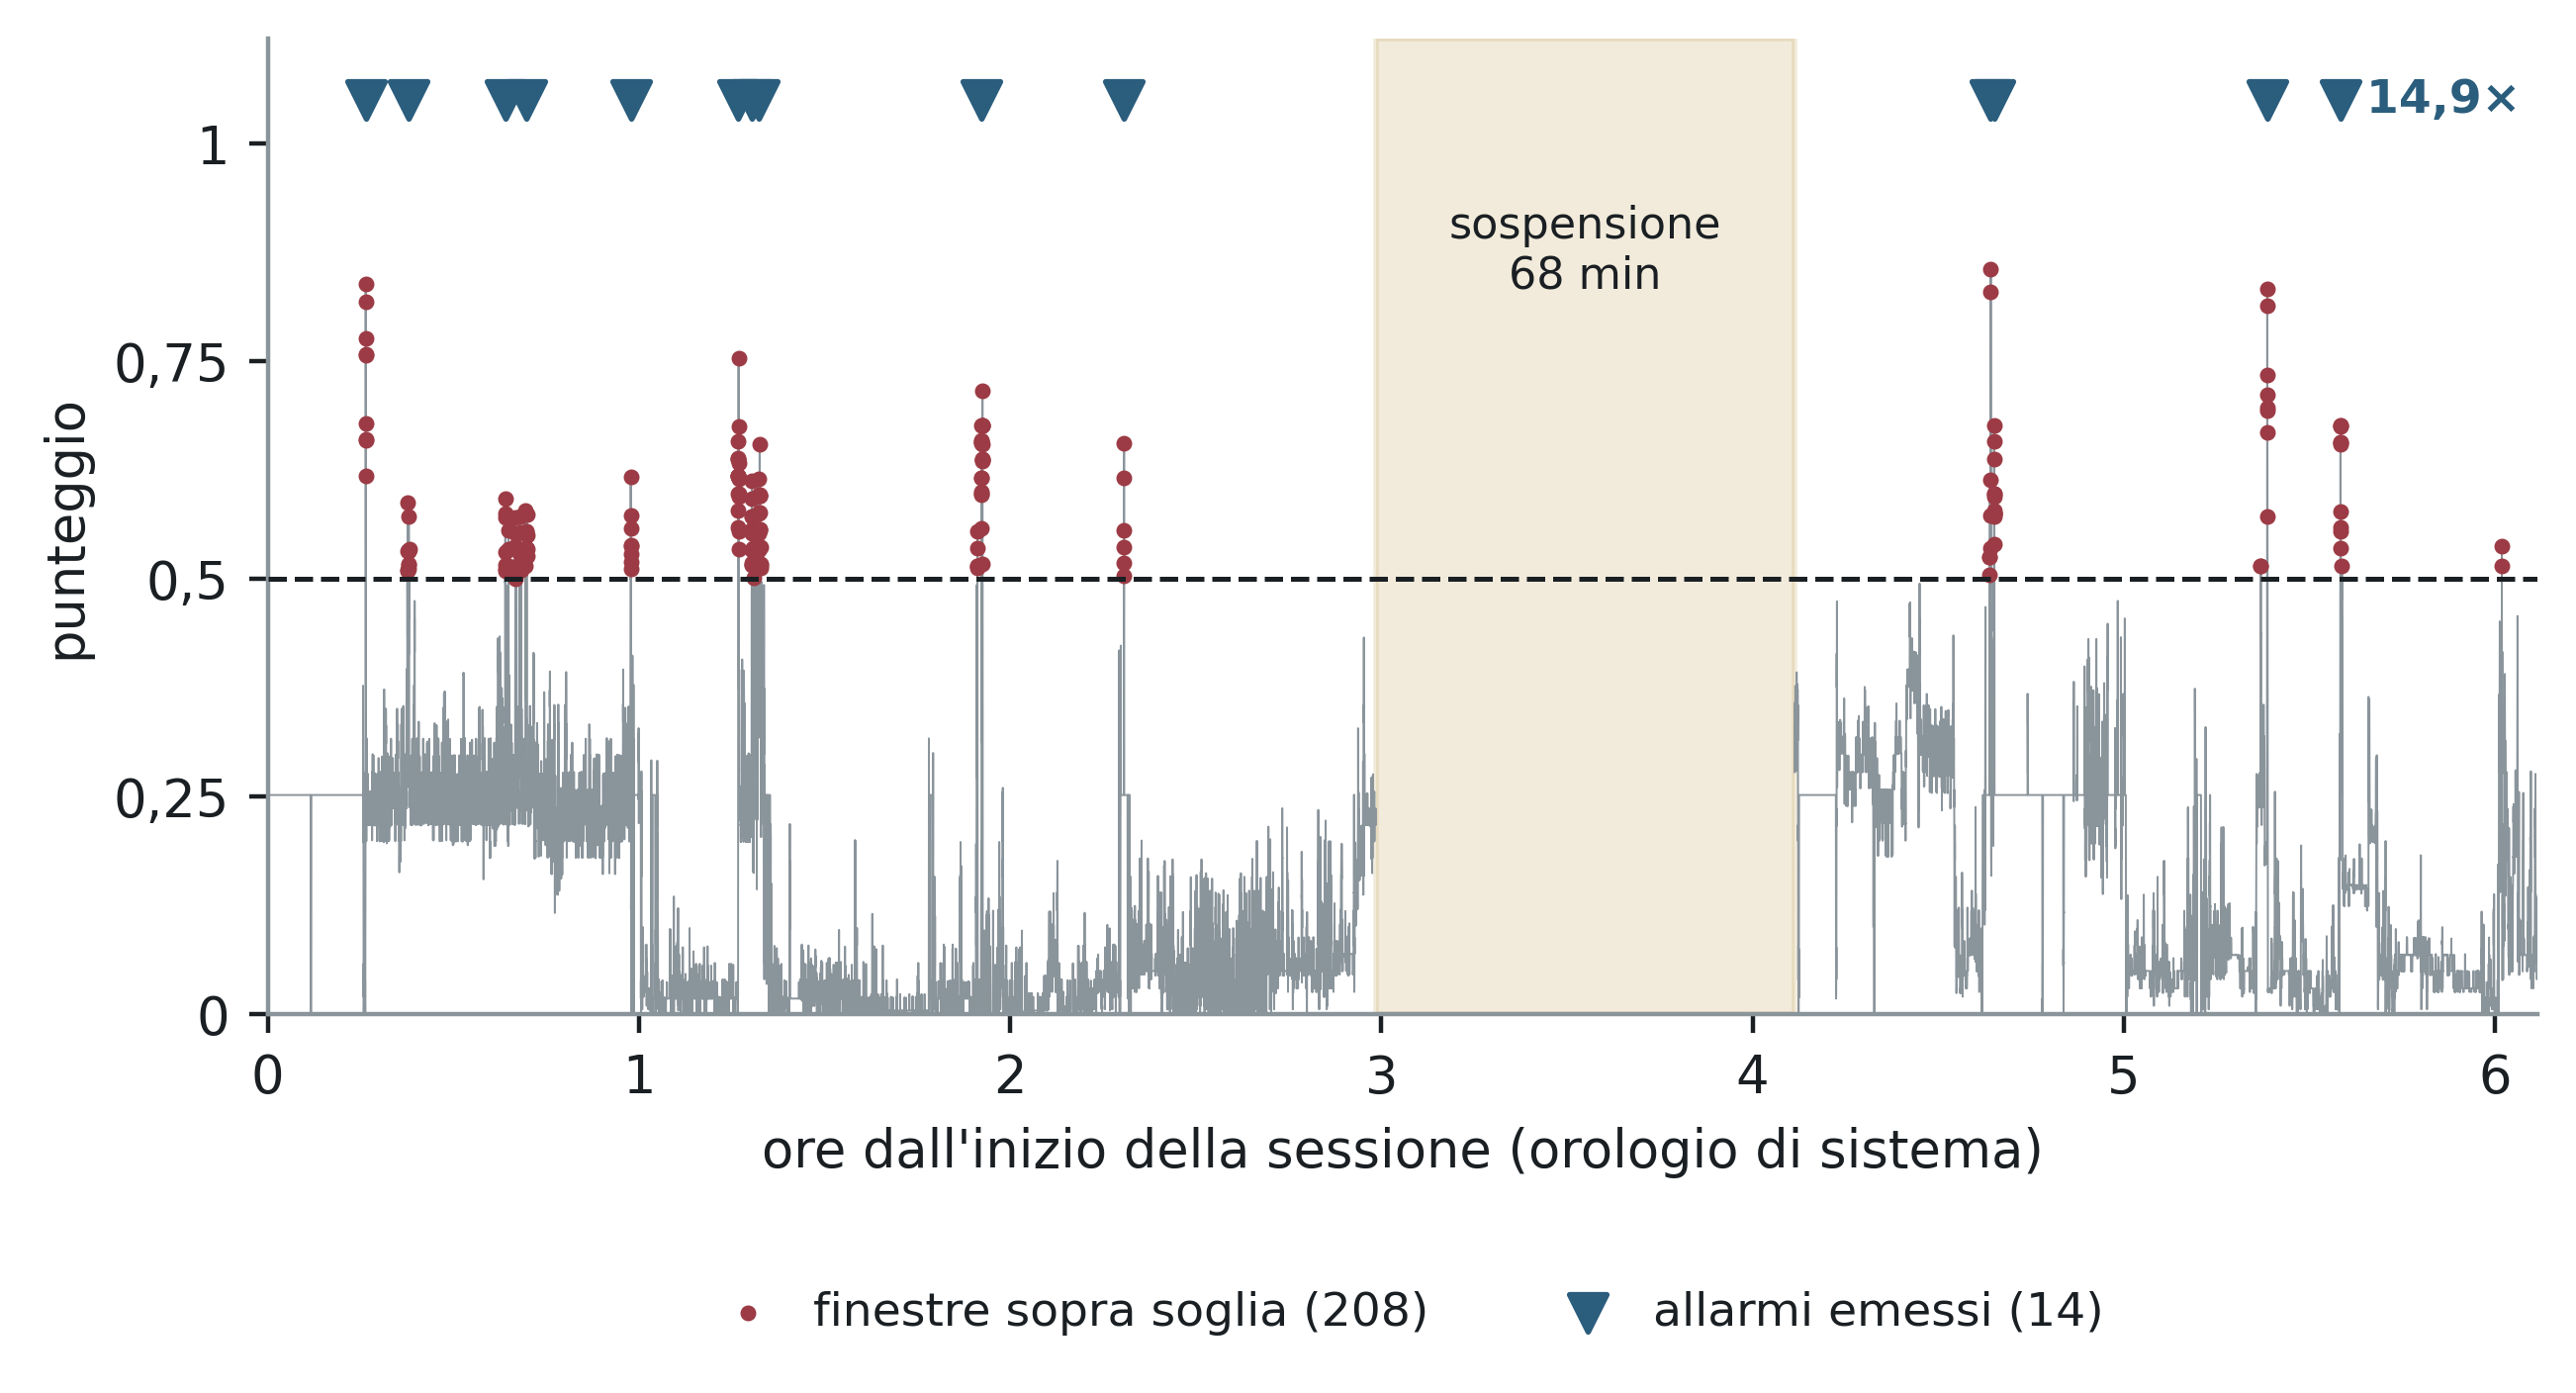
\includegraphics[width=.96\textwidth]{figure/fig_sessione.png}
\caption{Andamento del punteggio durante una sessione prolungata. I punti
sopra la soglia rappresentano le singole finestre positive, mentre i triangoli
indicano gli eventi effettivamente generati dopo l'applicazione della regola di
persistenza e della sospensione di 30~s. \textbf{I valori riportati riguardano
questa singola sessione} --- 208 finestre e 14 eventi, cioè un rapporto di
14,9 --- e non vanno confusi con il rapporto di 44,8 calcolato sull'insieme di
tutte le registrazioni.}
\label{fig:sessione}
\end{figure}

Nella sessione mostrata si osservano 208 finestre sopra soglia ma soltanto 14 eventi di allarme, con un rapporto pari a 14,9. \textbf{Il rapporto non è una costante del sistema}: dipende da quanto sono lunghe le sequenze di punteggi elevati, e varia quindi fra le registrazioni. Sulle singole sessioni assume valori compresi indicativamente fra 12 e 15; il valore aggregato di 44,8 è invece il rapporto fra due somme, ed è dominato dalle registrazioni con le raffiche più lunghe. Le due quantità rispondono a domande diverse e non vanno confrontate direttamente. Per questo motivo i conteggi a livello di finestra non devono essere utilizzati come numero di falsi allarmi.

Durante il funzionamento vengono quindi mantenute due grandezze distinte. Il \textbf{numero di eventi per unità di tempo} descrive quante segnalazioni riceverebbe effettivamente l'utente ed è confrontabile con i sistemi riportati in letteratura: è la metrica operativa principale di questo capitolo. La \textbf{quota di tempo trascorsa sopra soglia}, o equivalentemente il conteggio delle finestre positive, descrive invece quanto a lungo il sistema rimane in uno stato compatibile con una caduta, ed è usata come misura diagnostica del comportamento del classificatore.

La seconda misura è utile soprattutto per gli errori persistenti. Una persona distesa su un divano per un'ora non produce un singolo evento breve ma uno stato che può mantenere il punteggio elevato per un periodo prolungato. La sospensione di 30~s riduce il numero di notifiche, ma non modifica il fatto che il classificatore continui a interpretare quella configurazione come positiva. La logica di soppressione delle raffiche è infatti progettata per \emph{eventi}: uno stato che dura non viene compresso, e in una casa con persone anziane il falso positivo dominante è uno stato.

\subsection{Richiamo e criteri di associazione degli eventi}
\label{sec:recall-campo}

La misura del richiamo in ambiente domestico richiede di stabilire quando un evento di allarme possa essere associato a una caduta annotata. Nelle registrazioni disponibili le cinque cadute simulate sono annotate soltanto al minuto e non è quindi noto con precisione l'istante in cui inizia ciascun evento.

Il risultato dipende di conseguenza da due parametri. Il primo è la tolleranza temporale utilizzata per associare un allarme all'orario annotato. Il secondo è la persistenza richiesta dalla regola di allarme.

La Tabella~\ref{tab:tolleranza} riporta il numero di cadute riconosciute al variare di questi due parametri.

\begin{table}[ht]
\centering
\caption{Cadute associate a un evento di allarme al variare della tolleranza
temporale e della persistenza richiesta. Sono riportati i conteggi assoluti:
con cinque eventi una percentuale sarebbe fuorviante.}
\label{tab:tolleranza}
\begin{tabular}{lcc}
\toprule
\textbf{Tolleranza} &
\textbf{Persistenza 1} &
\textbf{Persistenza 5} \\
\midrule
$\pm10$ s & 0/4 & 0/4 \\
$\pm30$ s & 2/5 & 1/5 \\
$\pm60$ s & 3/5 & 1/5 \\
$\pm90$ s & 4/5 & 1/5 \\
\bottomrule
\end{tabular}
\end{table}

Il valore di \textbf{quattro cadute rilevate su cinque} viene quindi ottenuto soltanto utilizzando una finestra di associazione molto ampia e accettando una singola finestra positiva come rilevamento. Applicando invece la regola operativa di cinque finestre consecutive, soltanto una delle cinque cadute genera un evento all'interno delle tolleranze considerate.

Una tolleranza molto ampia aumenta inoltre la probabilità di associare alla caduta un falso allarme avvenuto per un'altra attività. Questo problema è particolarmente importante quando il tasso di falsi allarmi è elevato: in un intervallo di alcuni minuti può essere presente una segnalazione anche senza una relazione causale con la caduta. Va aggiunto che l'annotazione dell'operatore è al minuto, quindi l'istante vero è noto a meno di sessanta secondi e già $\pm30$~s è generoso; e che una tolleranza di novanta secondi contraddice la motivazione clinica del Capitolo~\ref{cap:contesto}, secondo cui il danno dipende dal tempo trascorso a terra.

Per questo motivo il richiamo di campo non viene riportato come un singolo valore indipendente dal protocollo. Il numero di cadute riconosciute deve essere sempre accompagnato dalla tolleranza di accoppiamento e dalla persistenza utilizzate.

La numerosità costituisce un ulteriore limite, ed è il più serio. \textbf{Cinque cadute simulate non stimano una probabilità di rilevamento}: l'intervallo di confidenza al 95\% su quattro rilevamenti su cinque va da $0{,}28$ a $0{,}99$, e non permette quindi di distinguere in modo affidabile configurazioni che differiscono di una sola caduta. Per questa ragione, nel seguito del capitolo, nessuna configurazione viene dichiarata migliore di un'altra sulla base del solo conteggio delle cadute.

Durante questa verifica è stata inoltre individuata una discordanza fra l'analisi eseguita offline e il comportamento registrato sulla board. La prima procedura indicava due cadute riconosciute su cinque, mentre il dispositivo ne aveva segnalate quattro utilizzando lo stesso modello.

La differenza era dovuta a due cause. Nell'analisi offline venivano mediati i modelli prodotti dalla validazione incrociata, mentre sulla board viene utilizzato un modello riaddestrato sull'intero insieme disponibile. Inoltre, alle sessioni domestiche veniva applicato nuovamente il sottocampionamento utilizzato per portare UP-Fall da 18 a 9~fps, nonostante la board producesse già circa 7--8~fps. La frequenza veniva quindi dimezzata una seconda volta e la finestra da 22 campioni arrivava a coprire circa 5,5~s.

Una volta eliminate entrambe le differenze, l'analisi offline riproduce il comportamento registrato dal dispositivo. Questa verifica è necessaria prima di confrontare le configurazioni nelle sezioni successive: due procedure che guardano gli stessi dati non possono dare risultati diversi, e finché la discrepanza non è spiegata nessun confronto è valido.

\subsection{Latenza di rilevamento}
\label{sec:latenza}

Una seconda metrica operativa è il tempo che intercorre fra l'inizio della caduta e la generazione dell'allarme. Questa grandezza non può però essere misurata direttamente nelle sessioni disponibili, perché l'istante delle cadute è annotato soltanto al minuto, mentre il ritardo atteso è dell'ordine dei secondi: l'incertezza sull'istante vero arriva quindi a sessanta volte la quantità da stimare.

La prima finestra sopra soglia compare, nelle cadute riconosciute, a 11,8, 19,4, 27,7 e 32,3~s rispetto al minuto annotato. Questi intervalli non possono essere interpretati come latenze del sistema: sono il punto del minuto in cui la persona è caduta.

È invece possibile scomporre la latenza nelle componenti determinate dalla configurazione. Considerando la frequenza media di 8,02~fps osservata nella sessione, una finestra di 22 campioni e una persistenza pari a cinque finestre, si ottengono i valori della Tabella~\ref{tab:latenza}.

\begin{table}[ht]
\centering
\caption{Scomposizione della latenza di segnalazione \textbf{nel caso
conservativo}. Il totale vale \emph{se} la finestra deve riempirsi dopo
l'inizio della caduta, condizione che la misura empirica mostra non essere
richiesta.}
\label{tab:latenza}
\begin{tabular}{lrr}
\toprule
\textbf{Componente} & \textbf{Tempo} & \textbf{Quota} \\
\midrule
Elaborazione del fotogramma & 0,125 s & 3,2\% \\
\textbf{Riempimento della finestra} & \textbf{2,743 s} & \textbf{71,0\%} \\
Persistenza & 0,997 s & 25,8\% \\
\midrule
\textbf{Totale, caso conservativo} & \textbf{3,865 s} & \\
\bottomrule
\end{tabular}
\end{table}

Il contributo dominante è quindi il riempimento della finestra temporale: 2,743~s contro 125~ms di elaborazione del singolo fotogramma, cioè un \textbf{fattore ventidue}. La latenza di segnalazione è determinata principalmente dalle scelte temporali della pipeline e non dalla velocità del classificatore.

\emph{Il termine di elaborazione è stato corretto.} Fino all'8 settembre 2026 questa tabella riportava 0,038~s, cioè il costo per fotogramma della misura ritirata nella Sezione~\ref{sec:costo}, e ne ricavava un rapporto superiore a settanta. Alla cadenza effettivamente misurata il termine vale 0,125~s e il rapporto è ventidue: la conclusione --- la latenza dipende da come è fatta la finestra e non da quanto è veloce il dispositivo --- regge, il fattore no.

La Tabella~\ref{tab:latenza_sensibilita} isola il contributo di ciascuna scelta.

\begin{table}[ht]
\centering
\caption{Da che cosa dipendono i 3,865~s. Ogni riga muove un solo parametro a
partire dalla configurazione installata.}
\label{tab:latenza_sensibilita}
\begin{tabular}{lrr}
\toprule
\textbf{Configurazione} & \textbf{Caso conservativo} & \textbf{Variazione} \\
\midrule
Installata: $L=22$ a 8,02 fps, persistenza 5 & 3,865 s & --- \\
Persistenza 1, tutto il resto identico & 2,868 s & $-26\%$ \\
Finestra di 1,5 s, persistenza 1 & \textbf{1,625 s} & $\mathbf{-58\%}$ \\
Dispositivo dieci volte più veloce & 3,753 s & $-3\%$ \\
\bottomrule
\end{tabular}
\end{table}

\textbf{La persistenza costa un secondo, la finestra lunga ne costa un altro e un quarto, e il dispositivo un decimo di secondo.} Comprare hardware più veloce non recupera quindi la latenza: la recuperano soltanto scelte di progetto già discusse altrove per altre ragioni.

La persistenza introduce inoltre una variabilità aggiuntiva. Il valore di 0,997~s rappresenta il minimo necessario per ottenere cinque finestre consecutive, ma nelle due cadute per le quali la sequenza completa viene osservata l'intervallo reale è rispettivamente 1,70 e 1,28~s. La differenza dipende dalla presenza di finestre che scendono temporaneamente sotto soglia e fanno ripartire il conteggio.

Una misura diretta della latenza è invece possibile in laboratorio, dove l'etichetta è per fotogramma e le cadute sono cinquanta anziché cinque. Misurando dal primo fotogramma etichettato «caduta in corso» alla fine della finestra che fa scattare l'allarme, la mediana alla regola installata è \textbf{2,44~s}, con richiamo 0,90 su cinquanta riprese. \emph{Questo valore è una misura di benchmark e non descrive il comportamento domestico}, dove la latenza resta non misurabile con l'annotazione disponibile.

\section{Confronto fra benchmark e comportamento reale}
\label{sec:rovesciamento}

Una volta definite le metriche operative, è possibile confrontare direttamente il comportamento delle stesse configurazioni nel dataset di laboratorio e nelle registrazioni domestiche.

Il confronto non ha lo scopo di stabilire se le due valutazioni producano lo stesso valore numerico, perché le metriche e le prevalenze sono differenti. L'obiettivo è verificare se le differenze che appaiono piccole nel benchmark corrispondano effettivamente a differenze altrettanto piccole durante l'esercizio. Tutte le configurazioni confrontate utilizzano \textbf{la stessa soglia decisionale e la stessa regola di aggregazione degli eventi}: le differenze osservate non possono quindi essere attribuite alla logica di allarme.

\subsection{Confronto delle configurazioni nei due domini}

Sono considerate cinque configurazioni costruite progressivamente a partire dalla rappresentazione A3. A3h aggiunge la stima dell'altezza rispetto al pavimento; A3i introduce le grandezze integrali descritte nel Capitolo~\ref{cap:metodologia}; le configurazioni con controesempi includono inoltre esempi negativi raccolti nelle sessioni domestiche.

\paragraph{Una precisazione sulla storia di queste configurazioni.} Né l'altezza dal pavimento né i controesempi domestici erano presenti nella configurazione inizialmente portata sul dispositivo. Entrambi sono stati introdotti \emph{dopo} aver osservato gli errori commessi nelle prime sessioni domestiche, e vanno quindi presentati come revisione successiva alla validazione sul campo e non come scelte compiute a priori. La distinzione è rilevante perché una feature motivata dall'analisi degli errori non può essere valutata come se fosse stata scelta in modo indipendente da essi.

\begin{table}[ht]
\centering
\caption{Confronto delle configurazioni in laboratorio e nelle registrazioni
domestiche, a parità di soglia e di regola di decisione. La colonna domestica
riporta finestre sopra soglia per ora, perché questa è la grandezza
disponibile in modo omogeneo per tutte le configurazioni; il conteggio delle
cadute è assoluto.}
\label{tab:configurazioni}
\begin{tabular}{lccc}
\toprule
\textbf{Configurazione} &
\textbf{$F_2$ laboratorio} &
\textbf{Finestre/ora in casa} &
\textbf{Cadute} \\
\midrule
A3 & $0{,}898\pm0{,}075$ & 139,9 & 3/5 \\
A3h & $0{,}931\pm0{,}051$ & 70,4 & 2/5 \\
A3h + controesempi & $0{,}942\pm0{,}060$ & 2,1 & 2/5 \\
A3i & $0{,}943\pm0{,}064$ & 9,8 & 4/5 \\
A3i + controesempi & $0{,}953\pm0{,}055$ & 2,7 & 3/5 \\
\bottomrule
\end{tabular}
\end{table}

Nel benchmark tutte le configurazioni migliorano rispetto ad A3 e la differenza fra la configurazione iniziale e quella finale è pari a 0,055 di $F_2$. Questo scarto rimane però dello stesso ordine della dispersione fra soggetti.

Nelle registrazioni domestiche la differenza assume una scala completamente diversa. A3 produce 139,9 finestre positive all'ora, mentre A3i con controesempi ne produce 2,7. La riduzione è quindi pari a un fattore di circa \textbf{52}.

Il benchmark non produce quindi necessariamente un ordinamento opposto delle configurazioni --- un'affermazione sostenuta da una versione precedente di questo lavoro e ritirata dopo l'estensione a dieci soggetti. Il problema è piuttosto che \textbf{comprime una differenza molto grande nell'ambiente domestico in uno scarto che, nel laboratorio, rimane difficile da distinguere dalla variabilità fra soggetti}. L'effetto pratico è però lo stesso di un ordinamento errato: chi selezionasse la configurazione sulla base del solo $F_2$ di laboratorio non avrebbe alcuna ragione statistica per preferire A3i con controesempi ad A3, e installerebbe un sistema che produce cinquantadue volte i falsi allarmi.

Anche i due tipi di errore devono essere considerati separatamente.

\begin{table}[ht]
\centering
\caption{Falsi negativi e falsi positivi delle cinque configurazioni nella
valutazione LOSO su dieci soggetti. I conteggi sono cumulati sui dieci fold.}
\label{tab:errori_lab}
\begin{tabular}{lcccc}
\toprule
\textbf{Configurazione} & \textbf{$F_2$} &
\textbf{Recall} & \textbf{FN} & \textbf{FP} \\
\midrule
A3 & 0,898 & 0,929 & 45 & 172 \\
A3h & 0,931 & 0,962 & 22 & 137 \\
A3h + controesempi & 0,942 & 0,965 & 22 & 129 \\
A3i & 0,943 & 0,977 & 14 & 150 \\
A3i + controesempi & 0,953 & 0,980 & 14 & 124 \\
\bottomrule
\end{tabular}
\end{table}

\begin{figure}[htbp]
\centering
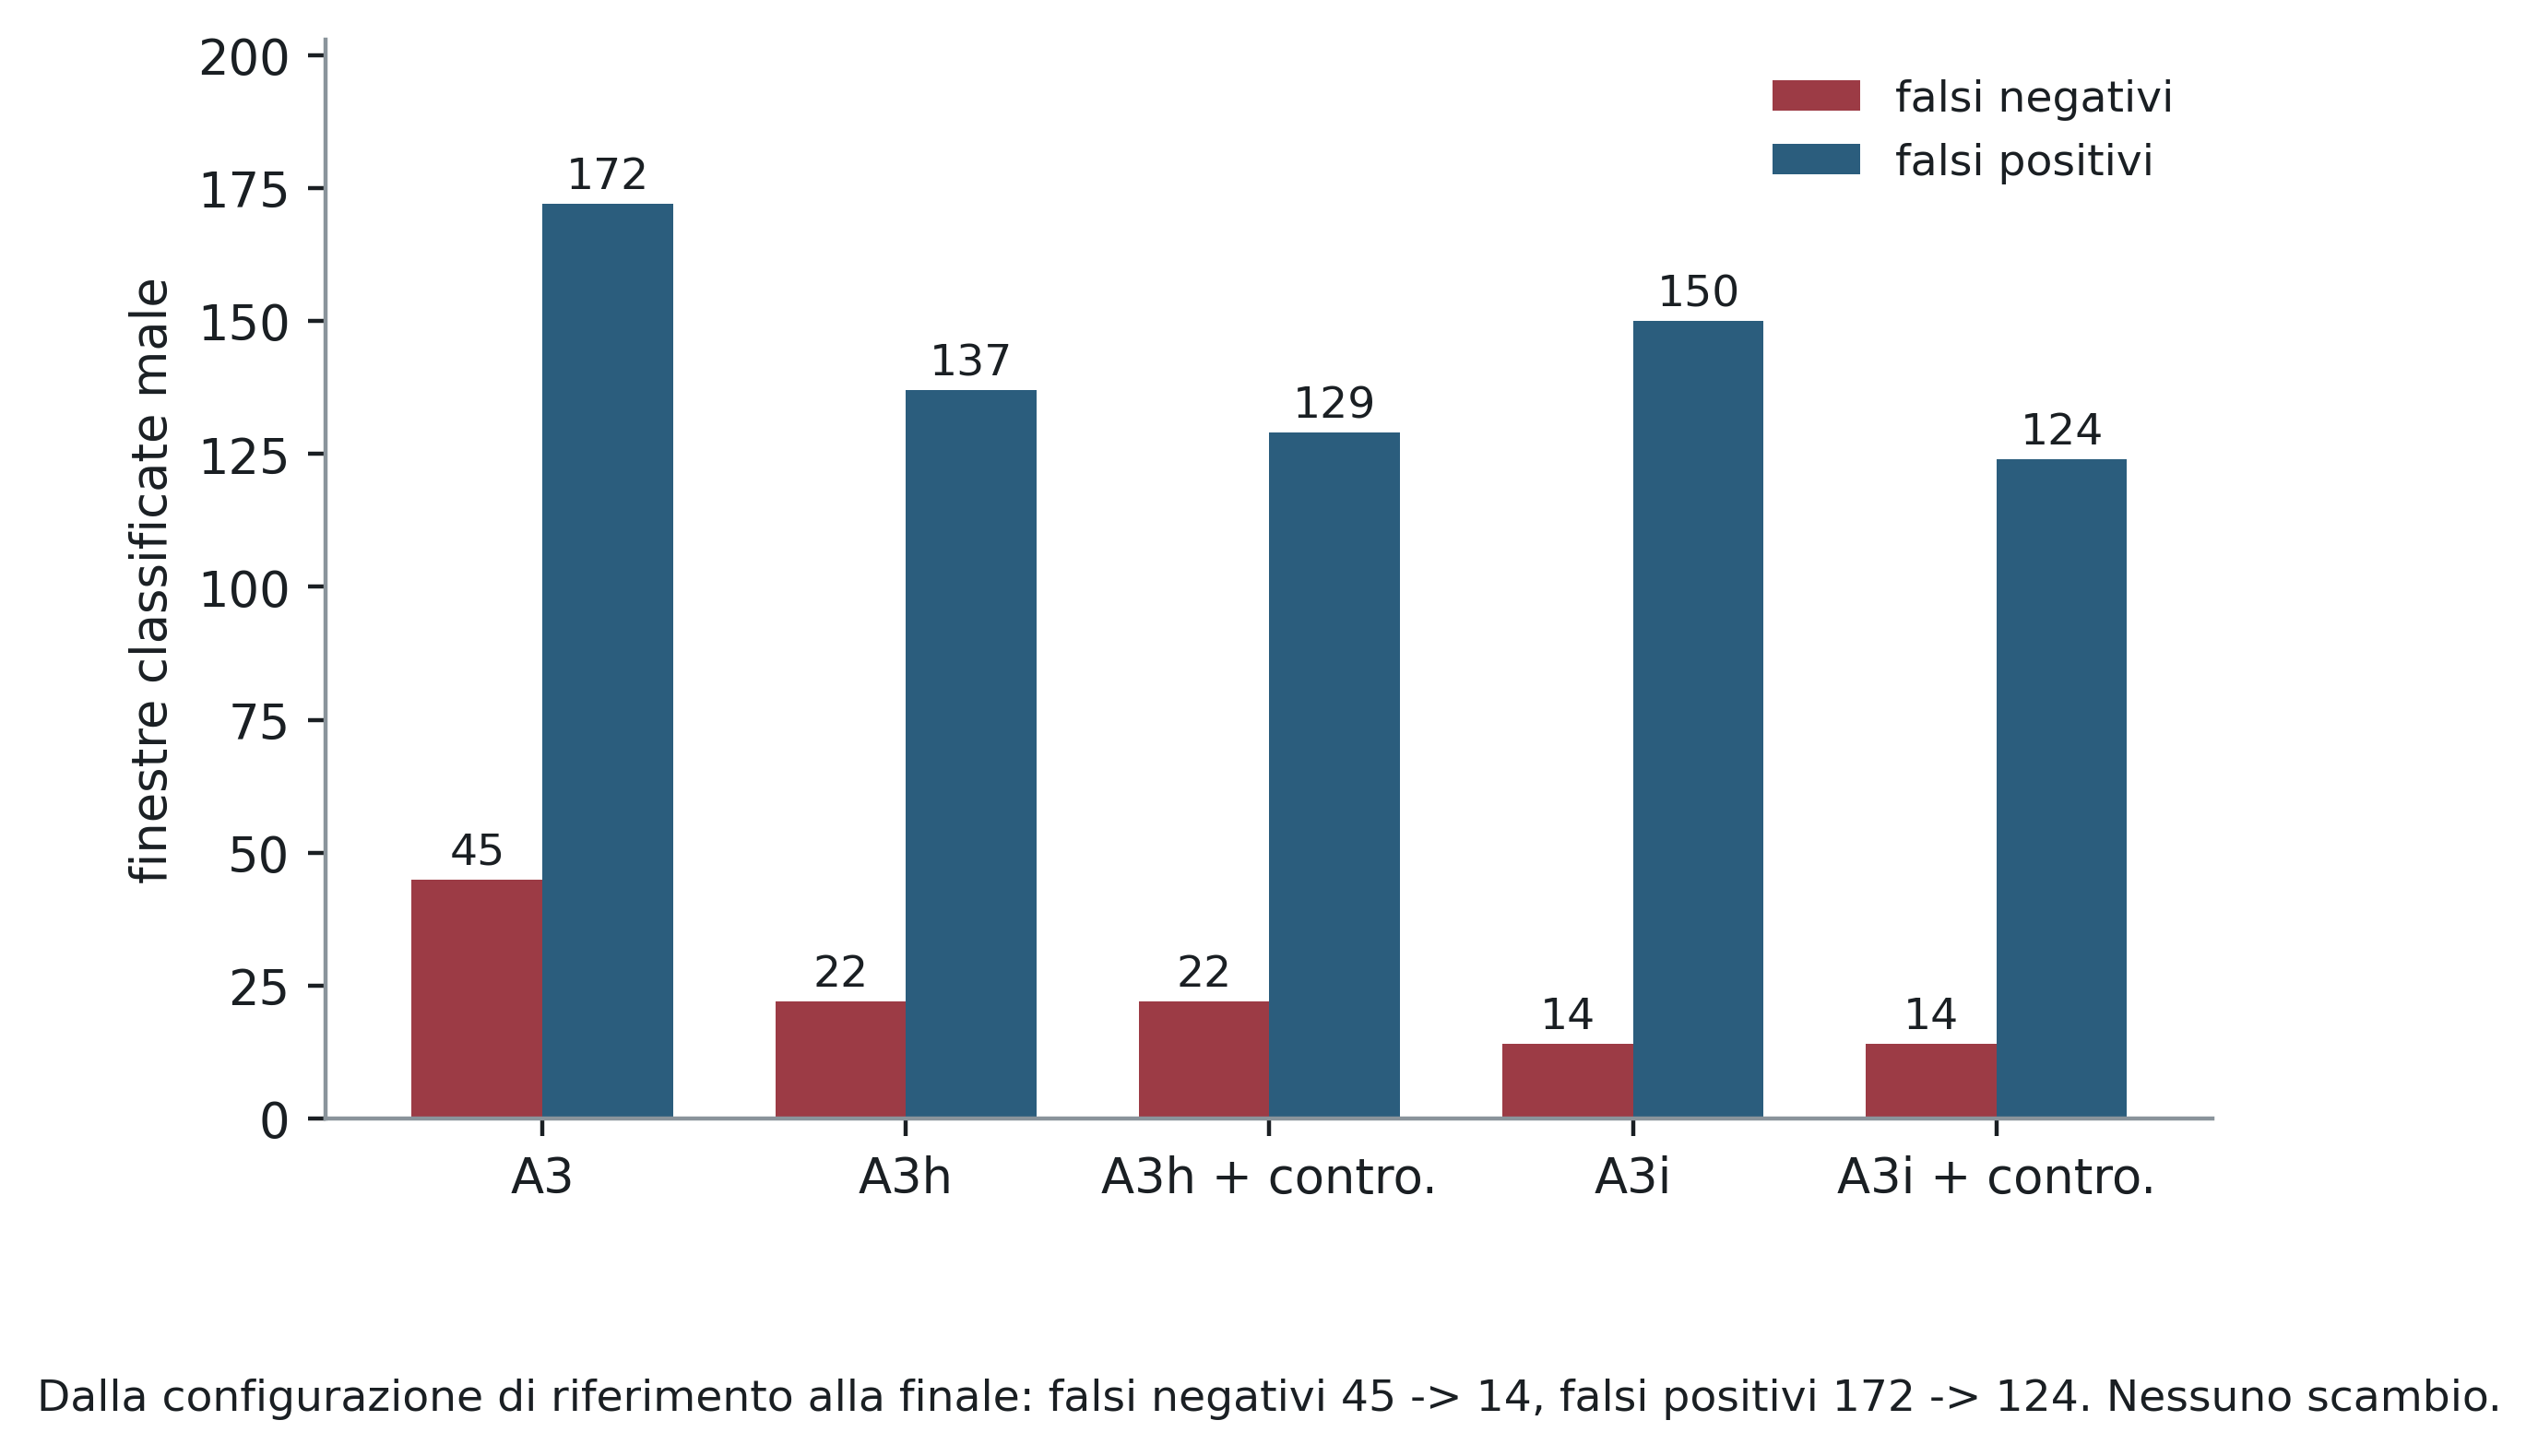
\includegraphics[width=.86\textwidth]{figure/fig_errori.png}
\caption{Falsi negativi e falsi positivi ottenuti dalle diverse
configurazioni nella valutazione di laboratorio, LOSO su dieci soggetti.}
\label{fig:errori}
\end{figure}

\textbf{In questo confronto, e alla soglia utilizzata}, la configurazione finale non migliora il richiamo a scapito dei falsi positivi: entrambi gli errori diminuiscono. Da A3 ad A3i con controesempi i falsi negativi passano da 45 a 14 e i falsi positivi da 172 a 124, mentre il richiamo sale da 0,929 a 0,980. L'osservazione va riferita a questo specifico confronto e a questa soglia, e non generalizzata: uno scambio fra i due errori compare invece in ambiente domestico, come mostrato più avanti.

La differenza principale fra laboratorio e casa non è quindi un semplice spostamento del compromesso fra precision e recall. È la diversa ampiezza con cui le modifiche introdotte vengono valorizzate dai due domini.

\subsection{Analisi delle differenze e trasferibilità dei controesempi}

La differenza osservata fra i due domini può essere ricondotta alla distribuzione delle attività negative. Nel dataset di laboratorio sono presenti persone in posizione orizzontale, ma nella maggior parte di questi casi il corpo si trova direttamente sul pavimento. Nelle registrazioni domestiche, invece, una parte consistente delle configurazioni orizzontali corrisponde a persone sdraiate su divani o altre superfici rialzate.

\begin{table}[ht]
\centering
\caption{Distribuzione qualitativa dei negativi orizzontali nei due domini.}
\label{tab:orizzontali}
\begin{tabular}{lcc}
\toprule
\textbf{Dominio} & \textbf{Quota approssimativa} &
\textbf{Posizione prevalente} \\
\midrule
Laboratorio & circa un quinto & pavimento \\
Ambiente domestico & circa metà & superficie rialzata \\
\bottomrule
\end{tabular}
\end{table}

La differenza è visibile anche nella stima dell'altezza del bacino. Considerando i negativi orizzontali, l'altezza mediana è pari a circa $+0{,}02$ lunghezze di torso nel dataset di laboratorio e a circa $+1{,}47$ nelle registrazioni domestiche.

Questo spiega perché una feature legata all'altezza rispetto al pavimento possa avere un effetto modesto su UP-Fall e diventare molto più utile in casa. Nel dataset, essere a terra non distingue necessariamente una caduta da una normale attività perché sono presenti azioni volontarie eseguite sul pavimento. In un'abitazione, al contrario, una persona orizzontale senza essere caduta si trova frequentemente su una superficie rialzata.

Se ne ricava un enunciato che si ritiene valga oltre il caso particolare:

\begin{quote}
Un insieme di verifica non può misurare un miglioramento su una condizione che
non rappresenta. Non si limita a sovrastimare le prestazioni: \textbf{comprime
differenze che in esercizio valgono ordini di grandezza fino a renderle non
dichiarabili}, e lo fa con la stessa apparente sicurezza con cui
distinguerebbe alternative davvero equivalenti.
\end{quote}

L'introduzione di controesempi domestici riduce fortemente i falsi positivi, ma presenta un possibile problema metodologico: gli esempi utilizzati durante l'addestramento provengono dalle stesse abitazioni nelle quali viene poi valutato il sistema.

Per verificare se il modello stia semplicemente imparando caratteristiche specifiche della stanza, il confronto viene ripetuto utilizzando i controesempi di una abitazione e valutando il sistema esclusivamente nell'altra.

\begin{table}[ht]
\centering
\caption{Trasferimento dei controesempi fra le due abitazioni.}
\label{tab:controesempi_cross}
\begin{tabular}{lcc}
\toprule
\textbf{Controesempi utilizzati} &
\textbf{Abitazione di test} &
\textbf{Eventi/ora} \\
\midrule
Nessuno / abitazione 2 & abitazione 1 & $0{,}342 \rightarrow 0{,}171$ \\
Nessuno / abitazione 1 & abitazione 2 & $1{,}781 \rightarrow 0{,}890$ \\
\bottomrule
\end{tabular}
\end{table}

Il tasso di allarme si riduce di circa un fattore due in entrambe le direzioni. Il beneficio non dipende quindi esclusivamente dalla stanza nella quale sono stati raccolti i controesempi.

Con due sole abitazioni non è comunque possibile parlare di generalizzazione a nuovi ambienti. I controesempi costituiscono più correttamente una forma di \textbf{adattamento al dominio mediante \emph{hard negatives}, con evidenza di trasferimento fra le due abitazioni considerate}: permettono al modello di osservare esempi negativi tipici del contesto domestico che non sono sufficientemente rappresentati nel dataset di laboratorio. Vanno quindi raccolti al momento dell'installazione, come si tara un sensore.

Il risultato mostra che una parte di questa informazione è trasferibile fra le due abitazioni considerate, ma non permette di stabilire quanto il beneficio rimanga invariato in una terza abitazione con arredamento, persone e geometria di ripresa differenti.

La riduzione dei falsi allarmi deve essere valutata insieme al numero di cadute riconosciute. I controesempi domestici riducono fortemente le finestre positive, ma nella configurazione A3i il numero di cadute riconosciute passa da quattro su cinque a tre su cinque. \textbf{Non è quindi un miglioramento: è uno scambio}, e in un sistema di sicurezza è lo scambio nella direzione che pesa di più.

Il comportamento risulta ancora più evidente considerando le tre definizioni del compito introdotte nel Capitolo~\ref{cap:risultati}. Le stesse registrazioni domestiche sono state rianalizzate utilizzando il compito evento, il compito stato e la loro combinazione, con la stessa soglia e la stessa regola di allarme.

\begin{table}[ht]
\centering
\caption{Comportamento delle tre definizioni del compito nelle registrazioni
domestiche, a parità di soglia e di regola di aggregazione.}
\label{tab:compiti_casa}
\begin{tabular}{lcc}
\toprule
\textbf{Compito} & \textbf{Eventi di allarme/ora} &
\textbf{Cadute rilevate} \\
\midrule
Evento & 1,6 & 3/5 \\
Stato & 29,5 & 0/5 \\
Allarme & 36,4 & 4/5 \\
\bottomrule
\end{tabular}
\end{table}

\begin{figure}[htbp]
\centering
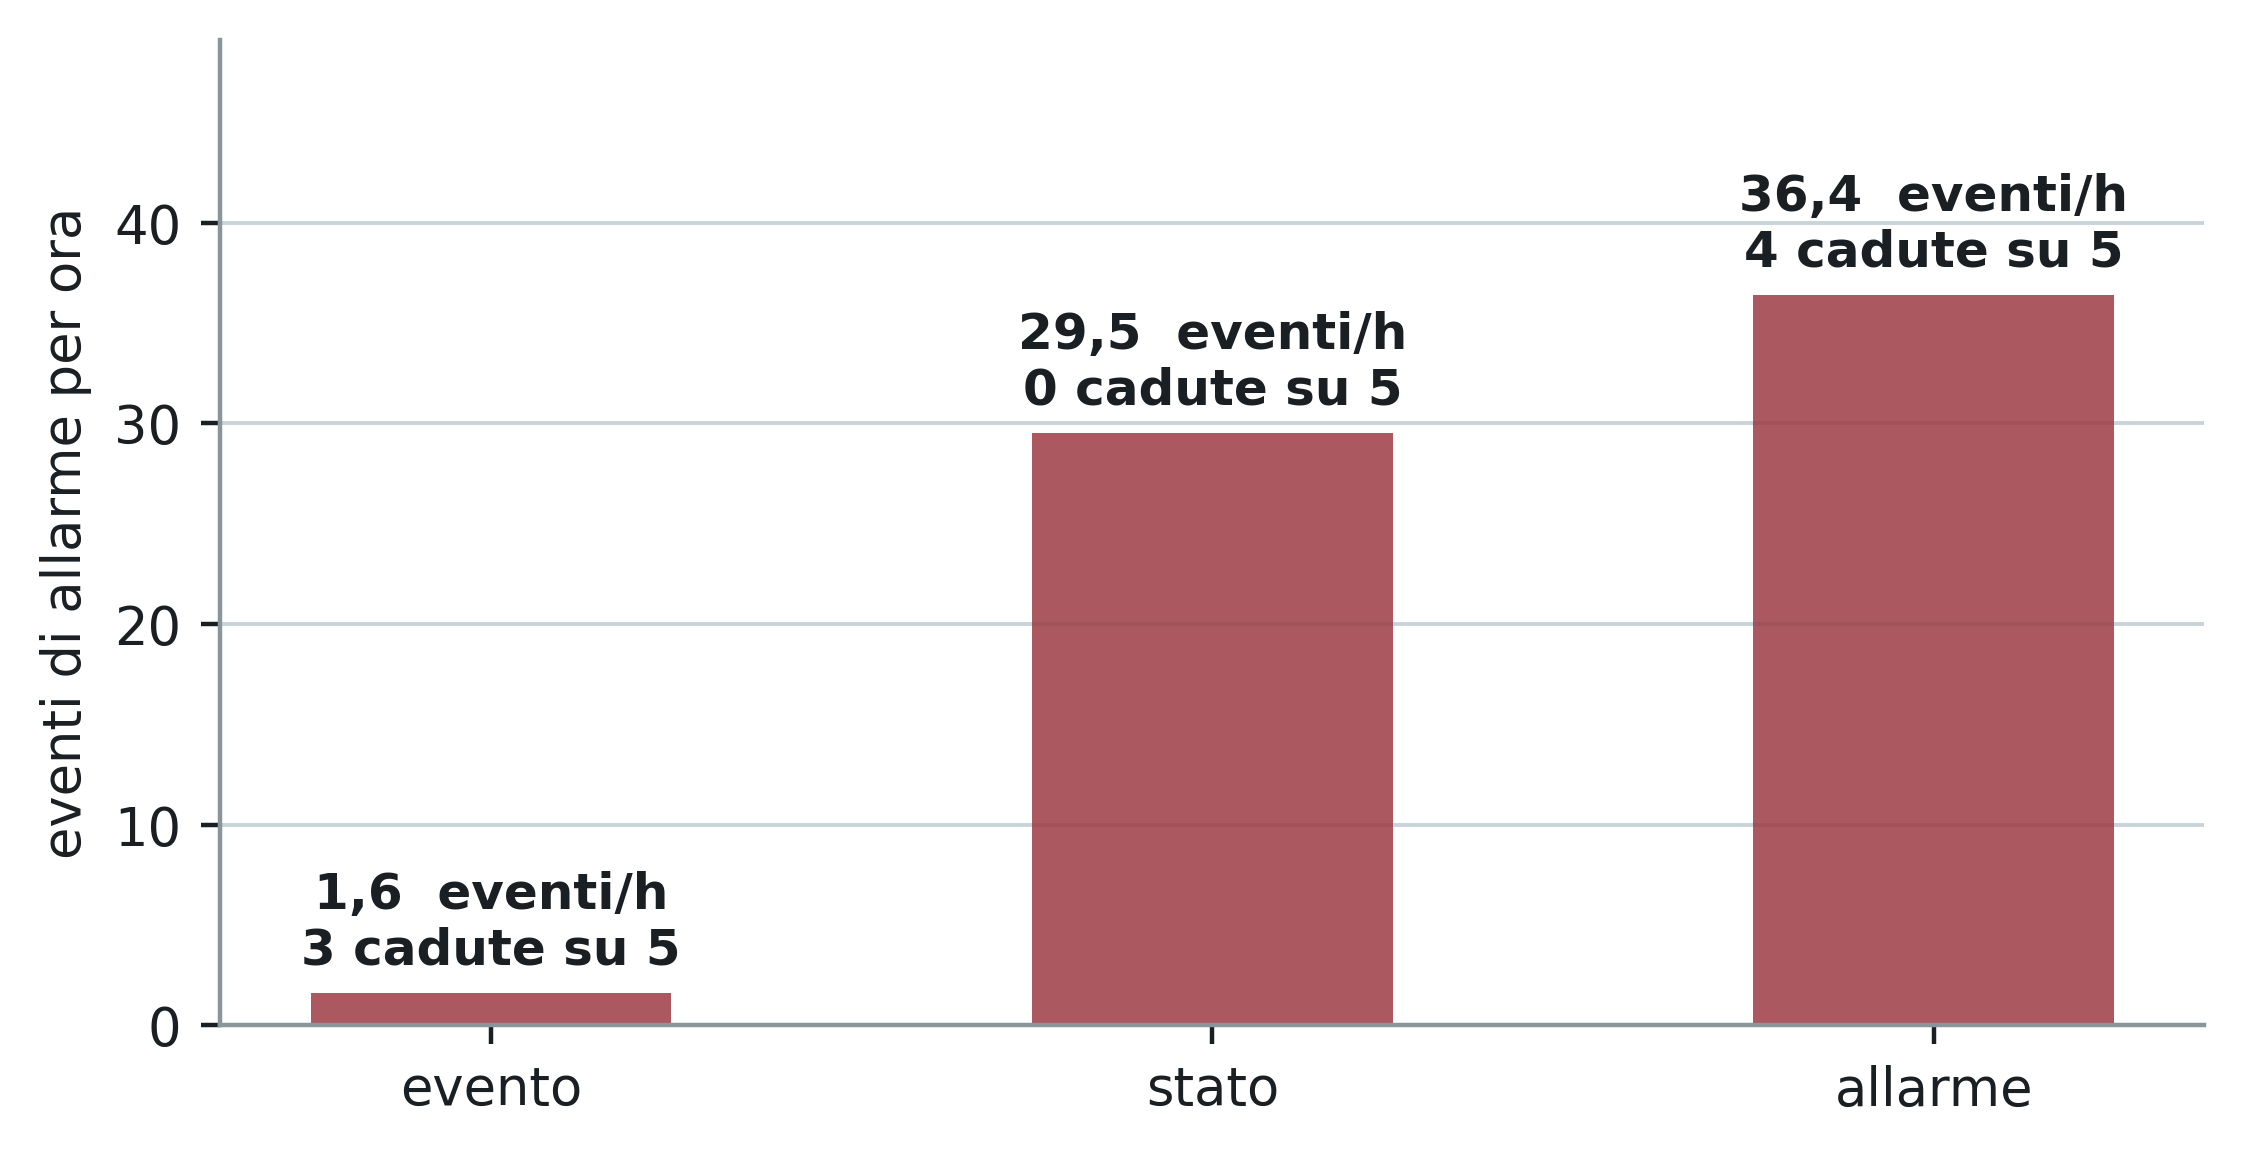
\includegraphics[width=.86\textwidth]{figure/fig_compiti_casa.png}
\caption{Confronto fra le tre definizioni del compito nelle registrazioni
domestiche, utilizzando la stessa regola di aggregazione degli eventi.}
\label{fig:compiti-casa}
\end{figure}

Il compito evento riduce il tasso di allarme di oltre un ordine di grandezza rispetto agli altri due. Il risultato è coerente con la valutazione del Capitolo~\ref{cap:risultati}, dove lo stesso compito non produceva falsi positivi sulle finestre corrispondenti a persone che si sdraiano volontariamente. \emph{Che la stessa scelta produca lo stesso ordine in due contesti così diversi è la corroborazione più solida di cui questo lavoro disponga.} Va notato inoltre che il compito \emph{stato}, che è la formulazione più diffusa in letteratura, è anche l'unico che in queste registrazioni non rileva alcuna caduta.

La riduzione non è però gratuita. Il compito evento riconosce tre delle cinque cadute considerate, mentre il compito allarme ne riconosce quattro. Anche in questo caso non è quindi possibile individuare una configurazione migliore considerando una sola metrica, né sulla base di una differenza di una sola caduta su cinque.

Con una numerosità così ridotta non è possibile stabilire con precisione quale dei due compromessi sia preferibile. Il risultato mostra però che la selezione di una configurazione destinata all'uso reale deve considerare contemporaneamente il richiamo e il numero di segnalazioni per unità di tempo.

\subsection{Effetto della finestra di accumulazione}
\label{sec:finestra-k}

Le grandezze integrali introdotte nel Capitolo~\ref{cap:metodologia} vengono calcolate su una finestra mobile di $K$ campioni. Il valore di $K$ determina quindi quanta storia del movimento viene incorporata nelle feature fornite al classificatore.

Questo parametro è stato variato mantenendo invariato il resto della pipeline, in modo da confrontarne l'effetto sia nel benchmark sia nelle registrazioni domestiche. I valori di laboratorio della scansione provengono dall'impianto sperimentale a cinque soggetti e sono quindi utilizzati principalmente per analizzare l'andamento.

\begin{table}[ht]
\centering
\caption{Effetto della lunghezza $K$ utilizzata per il calcolo delle
grandezze integrali nei due domini. I valori di laboratorio provengono
dall'impianto a cinque soggetti.}
\label{tab:kappa}
\begin{tabular}{rrrrr}
\toprule
$K$ &
\textbf{$F_2$ laboratorio} &
\textbf{FN} &
\textbf{Allarmi/ora in casa} &
\textbf{Cadute} \\
\midrule
5  & $0{,}859\pm0{,}125$ & 23 & --    & -- \\
15 & $0{,}928\pm0{,}048$ & 24 & 137,6 & 4/5 \\
22 & $0{,}963\pm0{,}016$ & 9  & 17,3  & 4/5 \\
31 & $0{,}980\pm0{,}020$ & 4  & 14,0  & 4/5 \\
45 & $0{,}987\pm0{,}008$ & 3  & 17,0  & 3/5 \\
\bottomrule
\end{tabular}
\end{table}

Il valore inizialmente utilizzato nella pipeline era $K=9$. La relativa riga della scansione appartiene ai risultati storici del progetto ma non è stata riprodotta nel controllo finale dei file di risultato; per questo motivo non viene utilizzata nella Tabella~\ref{tab:kappa} né nelle conclusioni che seguono.

Nel benchmark l'$F_2$ aumenta quasi regolarmente al crescere di $K$ e il valore più elevato viene raggiunto con $K=45$. Le registrazioni domestiche mostrano però un comportamento differente. Passando da $K=31$ a $K=45$ il numero di allarmi torna ad aumentare e le cadute riconosciute scendono da quattro a tre su cinque.

Se il parametro venisse scelto utilizzando soltanto il valore di $F_2$ in laboratorio, la configurazione selezionata sarebbe quindi $K=45$. Il comportamento in casa indica invece che l'aumento della memoria temporale oltre $K=31$ non produce un ulteriore beneficio operativo. \emph{È lo stesso fenomeno della sezione precedente, osservato però su un singolo iperparametro invece che su un intervento progettuale: il caso in cui è meno atteso e più facile da ignorare.}

Con $K=31$ le grandezze integrali utilizzano una storia temporale più lunga della finestra di classificazione. Questo non introduce informazione futura: le feature vengono calcolate soltanto utilizzando campioni già osservati e l'accumulazione viene azzerata fra registrazioni indipendenti e a ogni perdita della posa. Il sistema rimane quindi causale.

\paragraph{Quanto dura $K$, e perché non è lo stesso numero ovunque.} $K$ è un conteggio di fotogrammi e non una durata, e il tempo che rappresenta dipende dalla cadenza di chi lo produce. In estrazione le grandezze integrali sono calcolate sullo stream completo a circa 18~fps: $K=31$ corrisponde quindi a \textbf{1,72~s}, e il campo di ricezione complessivo --- accumulazione più finestra di decisione --- vale circa \textbf{4,2~s}. Sul dispositivo, che elabora fotogrammi consecutivi alla frequenza misurata di circa 7,3~fps, gli stessi 31 fotogrammi coprono invece \textbf{4,3~s}. Le grandezze integrali riassumono quindi in esercizio un intervallo di tempo circa due volte e mezzo più lungo di quello su cui il modello è stato addestrato. Esprimere $K$ come durata, e ricavarne il conteggio dalla cadenza osservata, è la correzione naturale e non è stata applicata nella configurazione qui riportata: costituisce un limite dichiarato del sistema installato.

Questo esperimento conferma quindi, anche per un singolo iperparametro, che la configurazione con il valore più elevato nel benchmark non coincide necessariamente con quella che produce il comportamento più utile durante l'esercizio.

\section{Modalità di fallimento e limiti osservati}
\label{sec:modi-fallire}
\label{sec:limiti-operativi}

Le sessioni in ambiente domestico hanno permesso di osservare alcune modalità di fallimento che non emergono direttamente dalla valutazione sui dataset. Questi casi riguardano sia il modello sia il funzionamento prolungato del dispositivo.

\paragraph{Scarsa dipendenza del punteggio dalla dinamica.}

La presenza di falsi allarmi su persone distese suggeriva inizialmente che il classificatore non utilizzasse in modo sufficiente l'informazione temporale. La correlazione misurata fra il punteggio prodotto e il movimento effettivo presente nella finestra è risultata pari a $+0{,}139$, quindi molto ridotta.

L'analisi successiva ha mostrato che il problema non era dovuto soltanto all'architettura del classificatore, ma alla rappresentazione fornita in ingresso. Le derivate istantanee risultavano sensibili al rumore della posa e non mantenevano una descrizione stabile della dinamica. Questa osservazione ha motivato l'introduzione delle grandezze integrali descritte nel Capitolo~\ref{cap:metodologia}.

\paragraph{Tracciamento di più persone.}

La pipeline è stata estesa per mantenere un'identità e uno stato delle feature separati per ciascuna persona osservata. Nell'unica sequenza disponibile con due persone contemporaneamente visibili, composta da 291 fotogrammi, non sono stati osservati scambi di identità.

La prova è però troppo breve per costituire una validazione completa. UP-Fall contiene una sola persona nella quasi totalità dei fotogrammi e non permette quindi di verificare sistematicamente il tracciamento multi-persona. \emph{La capacità che serve davvero in una casa è precisamente quella che nessun dato di laboratorio disponibile può misurare}, e questa rimane una delle differenze più rilevanti fra l'ambiente di laboratorio e una possibile installazione domestica.

La presenza di più persone produce inoltre un costo computazionale aggiuntivo. Lo stimatore esegue infatti la parte di stima dei landmark separatamente per ciascun soggetto rilevato. Nelle prove effettuate il frame rate passa da circa 7,5~fps con la stanza vuota a circa 4~fps con una persona e può scendere a 2--3~fps con due persone.

A queste frequenze una finestra di 22 campioni copre un intervallo temporale molto maggiore di quello utilizzato durante l'addestramento. Il problema non è quindi soltanto la riduzione della frequenza, ma anche il disallineamento fra la densità temporale del training e quella osservata in esercizio --- lo stesso fenomeno descritto per $K$ nella sezione precedente, qui indotto dal numero di persone in scena.

\paragraph{Filtro geometrico.}

È stata verificata anche la possibilità di inserire durante l'addestramento un vincolo geometrico basato sull'angolo del tronco, derivato dal \emph{Physics Guard} utilizzato nel prototipo iniziale.

Con una soglia pari a $110^\circ$ il numero di falsi positivi scende da 141 a 65. La recall diminuisce però da 0,941 a 0,872 e il numero di falsi negativi aumenta. Il filtro riduce quindi un tipo di errore introducendone altri in una direzione poco favorevole per un sistema di sicurezza. Per questo motivo non viene mantenuto nella configurazione finale, tanto più che i controesempi ottengono un effetto analogo sui falsi positivi senza costare richiamo.

\paragraph{Sospensione automatica del dispositivo.}

Una delle sessioni prolungate ha evidenziato che il sistema operativo poteva sospendere la board dopo un periodo di inattività anche quando il dispositivo era alimentato dalla rete. Nella registrazione rappresentata in Figura~\ref{fig:sessione} l'interruzione dura circa 68 minuti.

Il problema non provocava la terminazione del programma. Al risveglio la registrazione riprendeva normalmente e la scrittura della traccia proseguiva.

Il conteggio del tempo utilizzava però un cronometro monotono, che durante la sospensione non avanza. Al termine la sessione dichiarava quindi la durata richiesta anche quando una parte consistente dell'intervallo non era stata osservata, confrontando di fatto il tempo di esecuzione con se stesso. \emph{È il difetto più insidioso fra quelli osservati, perché non si manifesta come un errore}: la sessione sembra riuscita, e una prova notturna non sorvegliata avrebbe prodotto un tasso di allarmi eccellente e privo di significato.

Il difetto è stato individuato confrontando l'orologio di sistema con il cronometro monotono, e la correzione consiste nel disattivare la sospensione automatica. Il registratore riporta ora entrambi gli orologi e ne dichiara la differenza. Nella sessione ripetuta il 6 settembre i due valori coincidono a meno di 3,4~microsecondi su 4,59~ore di esercizio continuo: la sospensione non si è verificata, e questo risulta verificato anziché supposto.

\paragraph{Interruzione della cattura.}

Il dispositivo di acquisizione può essere rienumerato dal sistema operativo, con \texttt{/dev/video0} che diventa \texttt{/dev/video1}, tipicamente al risveglio o dopo un'instabilità del bus. Anche in questo caso il programma non termina: in assenza di sorveglianza la sessione prosegue fino al termine senza acquisire immagini. Nella sessione del 6 settembre si sono osservate due interruzioni della telecamera, per complessivi 5,1~secondi, entrambe recuperate automaticamente.

\paragraph{Che cosa una prova di durata non dimostra.}

Nella sessione del 6 settembre il sistema ha generato 14 eventi in 4,59~ore, pari a 3,1 eventi all'ora. Questi vanno riportati come \emph{eventi generati dal sistema} e non come falsi positivi: il registratore utilizzato in quella prova non salvava immagini, e in assenza di immagini non è possibile stabilire che cosa sia effettivamente accaduto in quei momenti. Nella stessa sessione la quota di fotogrammi con posa valida è pari al 35,1 per cento e non risulta alcuna caduta messa in scena. Si tratta quindi di una misura di durata e di costo, non di una misura di rilevamento. Il registratore è stato successivamente modificato per salvare nuovamente una sequenza di immagini di $\pm 10$~secondi attorno a ciascun allarme, per cui la verifica dei singoli eventi sarà possibile a partire dalla prossima sessione.

% =====================================================================
% LA CODA E' RICOSTRUITA il 9 settembre: dalla parola «normalmente» in
% poi le parole sono di chi ricostruisce, non quelle consegnate. Da
% confrontare con l'originale di Overleaf.
%
% I FATTI SONO PRESI DAL REGISTRO, non inventati:
%   - l'orologio monotono che non avanza durante la sospensione, e la
%     sessione che dichiara la durata confrontando il tempo con se stesso
%     (ISS-130, gia' descritto nel Cap5 del repository);
%   - la sessione del 6 settembre, EXP-024: 4,59 ore, scarto fra i due
%     orologi 3,4 microsecondi, nessuna sospensione, due interruzioni
%     della telecamera per 5,1 s in tutto riprese da sole, 119.928
%     fotogrammi, 7,26 fps, 35,1% di pose valide, 168 finestre sopra
%     soglia e 14 eventi = 3,05/ora;
%   - la rienumerazione di /dev/video0 in /dev/video1 (Cap5 del
%     repository, «La cattura si interrompe»);
%   - il registratore che torna a salvare +-10 s attorno all'allarme:
%     ISS-151, 9 settembre.
%
% I QUATTORDICI EVENTI sono chiamati «eventi generati dal sistema», che
% e' il punto 10 della lettera del relatore: senza immagini non si puo'
% dire se fossero falsi positivi.
%
% ATTENZIONE A NON CONFONDERE DUE SESSIONI. La §5.5 di questa stesura
% parla di «208 finestre e 14 eventi, rapporto 14,9»: quella e' la
% sessione di `fig:sessione`, cioe' quella CON la sospensione di 68
% minuti. La sessione del 6 settembre ha 168 finestre e 14 eventi. Il
% numero di eventi coincide per caso.
%
% NON VERIFICATO: che questa sia la coda che la candidata aveva scritto.
% E' la coda che i fatti registrati sostengono.
% =====================================================================
